\documentclass[a4paper,oneside,10pt]{book}
\usepackage{lastpage}
%
\usepackage{fancyhdr} 
%
%\usepackage{sfheaders} % set headers(sections, chapters, ... to sans sherif font)
%
\usepackage{amsmath}
%
\usepackage{draftcopy}
%
\usepackage{color}
%
\usepackage{listings}
%
\usepackage{graphicx}
%
\usepackage{tabulary}
\setlength{\tymin}{10pt}
\setlength{\tymax}{0.5\textwidth}
%


% Custom fonts -> uncomment and compile with XeLaTeX instead of LaTeX
%\usepackage{fontspec,xunicode}
%\defaultfontfeatures{Mapping=tex-text}
%\setsansfont[Scale=1]{Myriad Pro Light}
%\setromanfont[Scale=1.10]{LMRoman9 Regular}
%\setmonofont[Scale=1]{LMTypewriter10 Regular}

% Figures: path x width x angle x description x label
% eg. \image{image.pdf}{0.8}{0}{Global Sensor Network software architecture}{figure:gsn_architecture}
\newcommand{\image}[5]{
  \begin{figure} [!htp]
    \begin{center}
       \includegraphics[angle=#3, width=#2\textwidth]{#1}
       \caption{\label{#5} #4}
     \end{center}
  \end{figure}
}

% References
\newcommand{\figref}[1]{Figure~\ref{#1}}
\newcommand{\chapref}[1]{Chapter~\ref{#1}}
\newcommand{\annexeref}[1]{Appendix~\ref{#1}}
\newcommand{\tableref}[1]{Table~\ref{#1}}
\newcommand{\listingref}[1]{Listing~\ref{#1}}

% Listings
\definecolor{l_keyword}{rgb}{0.49,0,0.33} 
\definecolor{l_comment}{rgb}{0.49,0.62,0.75} 
\definecolor{l_string}{rgb}{0.16,0,1} 
\lstloadlanguages{Ruby,Java,XML,HTML}
% Default Settings
\lstset{
	basicstyle=\fontfamily{pcr}\fontseries{m}\fontshape{n}\small, % pcr | cmss
	keywordstyle=\color{l_keyword},
	commentstyle=\color{l_comment},
	stringstyle=\color{l_string},
	tagstyle=\color{black},
	tabsize=3,
	showstringspaces=false,
	captionpos=b,
	frame=none, %none, leftline, topline, bottomline, lines, single
	%numbers=left,
	%numberstyle=\fontfamily{pcr}\fontseries{m}\fontshape{n}\scriptsize,
	%numbersep=5pt,
	%stepnumber=1
}
% Per language Settings
\lstnewenvironment{rubycode}[1][]
	{\lstset{language=Ruby, #1}}
	{}
\lstnewenvironment{javacode}[1][]
	{\lstset{language=Java, #1}}
	{}
\lstnewenvironment{xmlcode}[1][]
	{\lstset{language=XML, #1}}
	{}
\lstnewenvironment{htmlcode}[1][]
	{\lstset{language=HTML, #1}}
	{}
\lstnewenvironment{bashcode}[1][]
	{\lstset{language=bash, #1}}
	{}

% Layout
\pagestyle{fancy}
\fancyhf{}
\fancyhead[L]{\nouppercase{\rightmark}}
\fancyhead[R]{\rule[-5pt]{0.5pt}{16pt}\makebox[21.3pt]{\thepage}}
\fancyfoot[L,R]{}
\renewcommand{\headrulewidth}{0.5pt}
\addtolength{\headheight}{4pt}
\addtolength{\voffset}{-15pt}
\addtolength{\textheight}{30pt}
\addtolength{\headwidth}{65pt}
\addtolength{\textwidth}{65pt}
\addtolength{\oddsidemargin}{-25pt}
\addtolength{\evensidemargin}{-55pt}
%
\fancypagestyle{plain}{ 
	\fancyhead[L,R]{}
	\fancyhead[L]{}
	\fancyfoot[R]{\thepage}
	\renewcommand{\headrulewidth}{0pt}
}
% 
\newcommand{\clearemptydoublepage}{\newpage{\pagestyle{plain}\cleardoublepage}}
%
\sloppy
\setlength{\parskip}{0.5\baselineskip} 

% Misc
\newcommand{\todo}[1]{\textcolor{red}{#1}}


\draftcopyName{Review V1}{135}
\title{Global Sensors Networks\thanks{The work presented in this paper was supported (in
    part) by the National Competence Center in Research on Mobile Information
    and Communication Systems (NCCR-MICS), a center supported by the Swiss
    National Science Foundation under grant no. 5005-67322 and by the L\'ion
    project supported by Science Foundation Ireland under grant no.
    SFI/02/CE1/I131.}}
\author{GSN Team}

%
% Document specific shortcuts
\newcommand{\gsn}{\textit{GSN}\xspace}
\newcommand{\vs}{\textit{VS}\xspace}
\newcommand{\vsd}{\textit{VSD}\xspace}
\newcommand{\wrapper}{\textit{Wrapper}\xspace}
\newcommand{\vsp}{\textit{VSP}\xspace}

\begin{document}
\maketitle

\frontmatter
\pagenumbering{roman}
%\setcounter{secnumdepth}{1}
\chapter{Abstract}
  With the price of wireless sensor technologies diminishing rapidly we can
  expect large numbers of autonomous sensor networks being deployed in the near
  future. These sensor networks will typically not remain isolated but the need
  of interconnecting them on the network level to enable integrated data
  processing will arise, thus realizing the vision of a global ``Sensor
  Internet.'' This requires a flexible middleware layer which abstracts from
  the underlying, heterogeneous sensor network technologies and supports fast
  and simple deployment and addition of new platforms, facilitates efficient
  distributed query processing and combination of sensor data, provides support
  for sensor mobility, and enables the dynamic adaption of the system
  configuration during runtime with minimal (zero-programming) effort. This
  paper describes the Global Sensor Networks (GSN) middleware which addresses
  these goals. We present GSN's conceptual model, abstractions, and
  architecture, and demonstrate the efficiency of the implementation through
  experiments with typical high-load application profiles. The GSN
  implementation is available from \url{http://gsn.sourceforge.net/}.	
  
  
  
\begin{table*}[!htp]
	\centering
	{\normalfont\footnotesize
	\begin{tabulary}{\textwidth}{|C|}%
	\hline
	\\
		\textbf This documentation is a work in progress \\
		\\
		If you find anything here to be incorrect, misleading or incomprehensible please contact us via the GSN Developers list at gsn-devel@lists.sourceforge.net.  \\
		\\
	\hline

	\end{tabulary}
	}
\end{table*}



 
 \newpage

% Table of contents
\tableofcontents	
\newpage	
\chapter{Related Publications}
Different parts of the work presented in this chapter are published in the form of articles in international conferences and workshops.
Parts of this chapter are also published in the form of internal technical reports.
\begin{itemize}
\item \emph{Infrastructure for data processing in large-scale interconnected sensor networks}, Karl Aberer , Manfred Hauswirth , Ali Salehi. Mobile Data Management (MDM), Germany, 2007.
\item \emph{GSN, Quick and Simple Sensor Network Deployment}, Ali Salehi, Karl Aberer. European conference on Wireless Sensor Networks (EWSN), Netherlands, 2007.
\item \emph{Zero-programming Sensor Network Deployment}, Karl Aberer , Manfred Hauswirth , Ali Salehi. Next Generation Service Platforms for Future Mobile Systems (SPMS), Japan, 2007.
\item \emph{A middleware for fast and flexible sensor network deployment}, Karl Aberer , Manfred Hauswirth , Ali Salehi. Very Large Data Bases (VLDB) Seoul, Korea, 2006.
\item \emph{Middleware support for the "Internet of Things"}, Karl Aberer , Manfred Hauswirth , Ali Salehi. 5. GI/ITG KuVS Fachgesprch "Drahtlose Sensornetze", Universitt Stuttgart, 2006.
\item \emph{The Global Sensor Networks middleware for efficient and flexible deployment and interconnection of sensor networks}, Karl Aberer , Manfred Hauswirth , Ali Salehi.
Technical Report, LSIR-2006-006.
\item \emph{Global Sensor Networks}, Karl Aberer , Manfred Hauswirth , Ali Salehi. Technical Report, LSIR-2006-001.
\end{itemize}
\newpage	


	% Chapters	
\mainmatter %start numbering with arabic numerals
%	\newpage
%	\pagenumbering{arabic}
	\setcounter{secnumdepth}{4}	
	\graphicspath{{chapters/ch-introduction/figures/}}
\chapter{Introduction}


\label{sec:introduction}

Until now, research in the sensor network domain has mainly focused on
routing, data aggregation, and energy conservation inside a single
sensor network while the integration of multiple sensor networks has
only been studied to a limited extent. However, as the price of
wireless sensors diminishes rapidly we can soon expect large numbers
of autonomous sensor networks being deployed. These sensor networks
will be managed by different organizations but the interconnection of
their infrastructures along with data integration and distributed
query processing will soon become an issue to fully exploit the
potential of this ``Sensor Internet.'' This requires platforms which
enable the dynamic integration and management of sensor networks and
the produced data streams.

The Global Sensor Networks (GSN) platform aims at providing a flexible
middleware to accomplish these goals.  GSN assumes the simple model
shown in Figure~\ref{fig:setup}. A sensor network internally may use
arbitrary multi-hop, ad-hoc routing algorithms to deliver sensor
readings to one or more sink node(s). A sink node is a node which is
connected to a more powerful base computer which in turn runs the GSN
middleware and may participate in a (large-scale) network of base
computers, each running GSN and servicing one or more sensor networks.

\begin{figure}
  \centering
  \includegraphics[width=0.5\columnwidth]{model}
  \caption{GSN model}
  \label{fig:setup}
\end{figure}

We do not make any assumptions on the internals of a sensor network
other than that the sink node is connected to the base computer via a
software wrapper conforming to the GSN API. On top of this physical
access layer GSN provides so-called \textit{virtual sensors} which
abstract from implementation details of access to sensor data and
define the data stream processing to be performed. Local and remote
virtual sensors, their data streams and the associated query
processing can be combined in arbitrary ways and thus enable the user
to build a data-oriented ``Sensor Internet'' consisting of sensor
networks connected via GSN.

\begin{comment} %following paragraph not really relevant in this context
In the following we start with a detailed description of the virtual
sensor abstraction in Section~\ref{sec:virt-sens-spec}, discuss GSN's
data stream processing and time model in
Section~\ref{sec:data-stre-proc}, and present GSN's system architecture
along with a discussion of essential implementation details
in Section~\ref{sec:system-architecture}. We
evaluate the performance of GSN in Section~\ref{sec:evaluation} and
discuss related work in Section~\ref{sec:relatedwork} before
concluding.
\end{comment}
\section{Terminology}

\begin{itemize}
	\item \textbf{Global Sensor Networks} (\gsn) defines both the project and the software described in this document. \\
	\item A \textbf{Wrapper} (\wrapper) is a piece of Java code that does the data acquisition for a specific type of device. \\
	\item A \textbf{Virtual Sensor} (\vs) is the main component in \gsn. It receives data from one or more \wrapper. It can combine their data, 
		process and finally store it. A \vs is defined in a single \vsd and combines different pieces of software 
	\begin{itemize}
		\item One \vsp
		\item Zero or Many \wrapper\textit{(s)}
	\end{itemize}
	\item A \textbf{Virtual Sensor Description file} (\vsd) is an XML file that contains the selection and the parametrization of the \vsp and \wrapper that compose a \vs.
		This file also contains the SQL statements that connect them together. \\
	\item A \textbf{Virtual Sensor Processing class} (\vsp) is a piece of Java code that process and stores the data upon reception from the \wrapper. \\
\end{itemize}

\section{Quick Start}

GSN (for Global Sensor Networks) is a software project that started in
2005 at EPFL in the LSIR Lab by Ali Salehi, under the supervision of
Prof. Karl Aberer. The initial goal was to provide a reusable software
platform for the processing of data streams generated by wireless
sensor networks. The project was successful, and was later reoriented
towards a generic stream processing platform.

GSN acquires data, filters it with an intuitive, enriched SQL syntax,
runs customisable algorithms on the results of the query, and outputs
the generated data with its notification subsystem.

GSN can be configured to acquire data from various data sources. The
high number of data sources in GSN allows for sophisticated data
processing scenarios. In the unlikely event that your data sources are
not supported, it is very easy to write a wrapper to make your hardware
work with GSN (you can find more information about this in chapter 5).

GSN offers advanced data filtering functionalities through an enhanced
SQL syntax. It is assumed that the reader has some knowledge of the
Standard Query Language (SQL). Using it for basic operations is fairly
intuitive and you should be able to start using it from the examples
provided in this document.

	\graphicspath{{chapters/ch-architecture/figures/}}

\chapter{GSN Architecture}

%\gsn is composed of three parts: data acquisition, data processing, and output
%dispatching (also called notification subsystem).


%\section{System architecture}
\label{sec:system-architecture}

GSN uses a container-based architecture for hosting virtual sensors.
Similar to application servers, GSN provides an environment in which
sensor networks can easily and flexibly be specified and deployed by
hiding most of the system complexity in the GSN Server.  Using the
declarative specifications, virtual sensors can be deployed and
reconfigured in GSN Servers at runtime. Communication and
processing among different GSN Servers is performed in a
peer-to-peer style through standard Internet and Web Services protocols. By
viewing GSN Servers as cooperating peers in a decentralized system,
we tried avoid some of the intrinsic scalability problems of many
other systems which rely on a centralized or hierarchical
architecture. Targeting a ``Sensor Internet'' as the long-term goal we
also need to take into account that such a system will consist of
``Autonomous Sensor Systems'' with a large degree of freedom and only
limited possibilities of control, similarly as in the Internet.

Figure~\ref{fig:NodeArchitecture} shows the layered architecture of a
GSN Server.

\begin{figure}%[htb]
  \centering
  \includegraphics[width=0.45\columnwidth]{NodeArchitecture}
  \caption{GSN Server architecture}
  \label{fig:NodeArchitecture}
\end{figure}

Each GSN server hosts a number of virtual sensors it is responsible
for. The virtual sensor manager (VSM) is responsible for providing
access to the virtual sensors, managing the delivery of sensor data,
and providing the necessary administrative infrastructure. The VSM has
two subcomponents: The life-cycle manager (LCM) provides and manages
the resources provided to a virtual sensor and manages the
interactions with a virtual sensor (sensor readings, etc.). The input
stream manager (ISM) is responsible for managing the streams,
allocating resources to them, and enabling resource sharing among them
while its stream quality manager subcomponent (SQM) handles sensor
disconnections, missing values, unexpected delays, etc., thus ensuring
the QoS of streams. All data from/to the VSM passes through the
storage layer which is in charge of providing and managing persistent
storage for data streams. Query processing in turn relies on all of
the above layers and is done by the query manager (QM) which includes
the query processor being in charge of SQL parsing, query planning,
and execution of queries (using an adaptive query execution plan). The
query repository manages all registered queries (subscriptions) and
defines and maintains the set of currently active queries for the
query processor.  The notification manager deals with the delivery of
events and query results to registered, local or remote virtual sensors. The
notification manager has an extensible architecture which allows the
user to largely customize its functionality, for example, having
results mailed or being notified via SMS.

The top three layers of the architecture deal with access to the GSN
server. The interface layer provides access functions for other GSN
servers and via the Web (through a browser or via web services).
These functionalities are protected and shielded by the access control
layer providing access only to entitled parties and the data integrity
layer which provides data integrity and confidentiality through
electronic signatures and encryption. Data access and data integrity
can be defined at different levels, for example, for the whole GSN
server or at a virtual sensor level.

In connection with RFID tags this ``plug-and-play'' feature of GSN
provides new and interesting types of mobility which we will
investigate in future work. For example, an RFID tag may store queries
which are executed as soon as the tag is detected by a reader, thus
transforming RFID tags from simple means for identification and
description into a GSN server for physically mobile queries which opens
up new and interesting possibilities for mobile information systems.

%\section{Self Identifying Devices}
%An interesting feature of GSN's architecture is the support for sensor
%mobility based on automatic detection of sensors and zero-programing
%deployment: A large number of sensors already support the IEEE 1451
%standard which describes a sensor's properties and measurement
%characteristics such as type of measurement, scaling, and calibration
%information in a so-called Transducer Electronic Data Sheet (TEDS)
%which is stored inside the sensor. When a new sensor node is detected
%by GSN, for example, by moving into the transmission range of a sink
%node, GSN requests its TEDS and uses the contained information for the
%dynamic generation of a virtual sensor description by using a virtual
%sensor description template and deriving the sensor-specific fields
%of the template from the data extracted from the TEDS. At the moment
%TEDS provides only that information about a sensor which enables
%interaction with it.  Thus for some parts of the generated virtual
%sensor description, e.g., security requirements, storage and resource
%management, etc., we use default values. Then GSN dynamically
%instantiates the new virtual sensor based on this synthesized
%description and all local and remote processing dependent on the new
%sensor is executed. This is done on-the-fly while GSN is running. The
%inverse process is performed if a sensor is no longer associated with
%a GSN node, e.g., it has moved away.


\section{Data Acquisition}

Before filtering and processing data, \gsn needs to receive it. \gsn considers two types of data sources: event-based and polling-based.
In the first case, data is sent by the source and a \gsn method is called when it arrives.
Serial ports, network (TCP or UDP) connections, wireless webcams fall in this case. In the latter one, GSN periodically asks the 
source for new data. This is the case of an RSS feed or a POP3 email account.

\subsection{\gsn Wrappers \label{gsn_wrappers}}

\gsn can receive data from various data sources. This is done by using so called
wrappers. They are used to encapsulate the data received from the data source
into the standard GSN data model, called a StreamElement. A StreamElement
is an object representing a row of a SQL table.
Each wrapper is a Java class that extends the AbstractWrapper parent class.
Usually a wrapper initializes a specialized third-party library in its constructor.
It also provides a method which is called each time the library receives data from
the monitored device. This method will extract the interesting data, optionally
parse it, and create one or more StreamElement(s) with one or more columns.
From this point on, the received data has been mapped to a SQL data structure
with fields that have a name and a type. \gsn is then able to filter this using
its enhanced SQL-like syntax. You will learn more about that in section \todo{TODO: Add proper reference}
A wrapper is implemented in a Java class. For simplicity, \gsn uses short
names to refer to these wrappers. These associations are defined in the file
conf/wrappers.properties. For now on it is assumed that you use the default
names provided at installation time.

The standard \gsn wrappers are documented in Appendix \ref{sec:quickref_wrappers}.

The development of \gsn wrappers is described in Appendix \ref{sec:developer-guide_wrappers}.

\subsection{Safe Storage \label{safe_storage}}

Some acquisition systems do not internally store the data produced until GSN can process it. For instance 
the TinyOS Serial Forwarder simply sends a copy of the incoming messages to all its alive listeners. If GSN is down 
at that time, the data produced will be lost. Safe Storage is specialy developed to handle that case.
Safe Storage runs in a separate process and it aims is to simply store persistently the incoming data until the GSN process can ask for them.

These two processes communicate together upon TCP sockets and could run on different machines. The Safe Storage process acts as 
a server and GSN processes as clients. This communication and the primary storage increase the delay between the data production and the 
final storage into GSN. This results in a tradeoff between the performances and the reliability.
Moreover, GSN can run both standard wrappers and Safe Storage wrappers at the same time.

\subsubsection{Software Architecture}

Safe Storage is generic and could be added to all the already existing wrappers.
However small modifications need to be done since the Safe Storage wrappers are split into the two following parts

\begin{itemize}
	\item The acquisition part that runs in the Safe Storage process
	\item The processing part that runs in the GSN process
\end{itemize}

The wrapper class that executes on the Safe Storage should be kept as simple as possible and must extend the
\inlinecode{gsn.acquisition2.wrappers.AbstractWrapper2} abstract class.
An implementation of this class must define the methods shown on the \listingref{listing:java:safestorage_methods_to_implement}.

\begin{javacode}[caption={Methods to implement for a Safe Storage Wrapper - Safe Storage Side}, label=listing:java:safestorage_methods_to_implement]
public abstract boolean initialize ()
public abstract void finalize ()
public abstract String getWrapperName () 
public abstract void run()
\end{javacode}

The class that executes on the GSN side should do the data processing and must extend the 
\inlinecode{gsn.acquisition2.wrappers.SafeStorageAbstractWrapper} abstract class.
An implementation of this class must define the methods shown on the \listingref{listing:java:safestorage_gsn_methods_to_implement}

\begin{javacode}[caption={Methods to implement for a Safe Storage Wrapper - GSN Side}, label=listing:java:safestorage_gsn_methods_to_implement]
public DataField[] getOutputFormat()
public boolean messageToBeProcessed(DataMsg dataMessage)
\end{javacode}

\subsubsection{Safe Storage configuration}

All the wrappers that are based on Safe Storage must set the list of parameters defined in \listingref{table:arch_safe_storage_parameters}.
The Safe Storage and Safe Storage controller port are defined in the \inlinecode{build.xml} file.

\begin{xmlcode}[caption={Safe Storage ports}, label=listing:xml:safestorage_ports]
   <property name="safe-storage-port" value="25000"/>
   <property name="safe-storage-controller-port" value="25012"/>
\end{xmlcode}

The \listingref{listing:xml:safestorage_vsd} shows an example of a \vsd that uses a Safe Storage \wrapper.

\begin{xmlcode}[caption={Sample of Email Notification VSD file}, label=listing:xml:safestorage_vsd]
<virtual-sensor name="ss_mem_vs" priority="10" >
	<processing-class>
		<class-name>gsn.vsensor.BridgeVirtualSensor</class-name>
		<output-structure>
			<field name="heap_memory_usage" type="bigint" />
			<field name="non_heap_memory_usage" type="bigint" />
			<field name="pending_finalization_count" type="int" />
		</output-structure>
	</processing-class>
	<description> Mem VS for Safe Storage Test </description>
	<life-cycle pool-size="10" />
	<addressing />
	<storage history-size="10"/>
	<streams>
		<stream name="data">
			<source alias="source" storage-size="1" sampling-rate="1">
				<address wrapper="ss_mem_processor">
					<predicate key="ss-host">localhost</predicate>
					<predicate key="ss-port">25000</predicate>
					<predicate key="continue-on-error">true</predicate>
					<predicate key="wrapper-name">mem2</predicate>
				</address>
				<query> select * from wrapper </query>
			</source>
			<query> select * from source </query>
		</stream>
	</streams>
</virtual-sensor>
\end{xmlcode}

\subsection{Safe Storage Wrappers Default parameters}

The parameters shown on the \listingref{table:arch_safe_storage_parameters} must be added to each \wrapper that support the 
Safe Storage feature. An example of \wrapper that use this feature is described in \chapref{tinyos-mig:wrapper}.

\begin{table*}[!htp]
	\centering
	{\normalfont\footnotesize
	\begin{tabulary}{\textwidth}{|C|C|C|C|J|}%
	\hline
		\multicolumn{5}{|c|}{\textbf{Safe Storage Parameters}} \\
	\hline
	\hline
		\textbf{Parameter Name} &
		\textbf{Type} &
		\textbf{Mandatory} &
		\textbf{Default} &
		\textbf{Description} \\
	\hline
	\hline
		ss-host &
		String &	
		Yes &
		None &
		The machine host name that runs the Safe Storage \\
	\hline
		ss-port &
		Integer &	
		Yes &
		None &
		The server port on which Safe Storage listen for connections \\
	\hline
		wrapper-name &
		String &	
		Yes &
		None &
		The Safe Storage side wrapper full classname (must extends \inlinecode{gsn.acquisition2.wrappers.AbstractWrapper2}) 
		or the short name from the \path{conf/safe\_storage\_wrappers.properties} file. \\
	\hline
		wrapper-keep-processed-ss-entries &
		Boolean &
		No &
		true &
		If this option is set to \inlinecode{true}, all the entries (processed or not) kept into the Safe Storage storage.
		If this option is set to \inlinecode{false}, the processed entries are removed from the Safe Storage storage once processed. \\
	\hline
		continue-on-error &
		Boolean &	
		No &
		true &
		Not yet implemented \\
	\hline
	\end{tabulary}
	}
	\caption{Safe Storage Parameters}
	\label{table:arch_safe_storage_parameters}
\end{table*}

\subsubsection{Use Cases}

When a virtual sensor that use a Safe Storage \wrapper is loaded into GSN,
a request is made to Safe Storage for the \wrapper. If the \wrapper is not already
created\footnote{In the current implementation, a Safe Storage \wrapper is identified by the following information:\newline{}
\inlinecode{<virtual-sensor-name>/<source-name>/<safe-storage-wrapper-short-name>}} 
this will create, initialize and run a new instance of the \wrapper in the Safe Storage process.
If the \wrapper was already running, it will be reused.

If the GSN process fails or is shut down, The Safe Storage \wrapper will continue to acquire the data. Once the GSN process is
restarted, all the data will be fetched from the Safe Storage DB.

If the Safe Storage process fails or is shut down, the data are not stored anymore and the GSN process will try periodically to 
connect to the Safe Storage process until the latter has been restarted.
When you restart the Safe Storage process, it will automatically create and start acquiring data for the wrappers that were loaded before.

\subsubsection{Safe Storage Management}

{
\setlength{\tymin}{10pt}
\setlength{\tymax}{0.8\textwidth}
\begin{table*}[!htp]
	\centering
	{\normalfont\footnotesize
	\begin{tabulary}{\textwidth}{|C|J|}%
	\hline
		\multicolumn{2}{|c|}{\textbf{Safe Storage ANT Tasks}} \\
	\hline
	\hline
		\textbf{Task Name} &
		\textbf{Description} \\
	\hline
	\hline
		start-acquisition &
		Start the Safe Storage process. The wrapper that were loaded during the last runs will be automatically resumed and will directly start acquiring data. \\
	\hline
		clean-acquisition &
		Delete all the Safe Storage permanent storage and flush the list of Wrappers to resume. Use this task with caution since it may delete unprocessed data. \\
	\hline
		stop-acquisition &
		Stop the Safe Storage process. \\
	\hline
	\hline
		\multicolumn{2}{|l|}{Use each of these tasks by typing in your terminal: \inlinecode{ant <Task Name>}} \\
	\hline
	\end{tabulary}
	}
	\caption{Safe Storage ANT Tasks}
	\label{table:safestorage_ant_tasks}
\end{table*}
}


\subsection{Safe Storage in Nutshell}

In order to coordinate the activities between the GSN and Safe Storage(SS), a custom protocol has defined. The GSN \textless-\textgreater SS protocol 
constitutes of the following messages:
\begin{description}
	\item[HelloMessage\footnote{Implemented by \texttt{gsn.acquisition2.messages.HelloMsg} class.}] is the first message sent from GSN to SS in order to represent the request to use a wrapper at the SS. In order to SS to instantiate the wrapper, SS has to know the following
	information about the requested wrapper:
	\begin{itemize}
		\item \texttt{wrapper's initialization parameters}, these are the original wrapper initialization parameters (exactly as they are specified in the virtual sensor file) sent from the GSN server to the SS. 
		\item \texttt{requester} or \emph{unique wrapper identifier} is a string which uniquely identifies the wrapper at the safe storage. As one safe storage component can be used to host multiple wrappers at the same time, SS has to create internal mapping between every request
		and the cooresponding wrapper at the SS. The mapping is used by the reconnection requests from the GSN (in the case of network disconnectivity or GSN crash) in order to resume the sensor data feed toward the GSN server.
		\item \texttt{continue-on-error} Which is a boolean ...
	\end{itemize}
	Once the HelloMessage received by the SS, SS stores the original HelloMessage into its internal storage. The reason behind this to 
	make sure SafeStorage as all the necessary information when its gets started. Whenever Safe Storage gets restarted, it resume the
	data acquisition process for all its previously active wrappers (without receiving HelloMessages).
\end{description}

\section{Data Filtering and Processing}

GSN provides two complementary mechanisms to work on data.
The first one is based on a SQL syntax enhanced with specialized semantics
for timed sliding windows and event counting.
The second one allows to manipulate data with specialized programs called
virtual sensors. GSN comes with a library of virtual sensors that you can use
without programming. 

GSN always processes the data according to a virtual sensor configuration.
If you only want to use the SQL filtering mechanism, without any data trans-
formation, you can use the BridgeVirtualSensor (see \ref{bridge:vsp}).
If you have more sophisticated needs, you can write your
own virtual sensor processing class (See appendix \ref{sec:vsp}).  If you don't want to use the SQL filtering mechanism, simply select all data
from the wrapper.

\subsection{Virtual Sensors}

%\section{Virtual sensors}
\label{sec:virt-sens-spec}


The key abstraction in GSN is the \textit{virtual sensor}. Virtual
sensors abstract from the implementation details of the data aource to sensor data
and correspond either to a data stream received directly from sensors
or to a data stream derived from other virtual sensors. A virtual
sensor can be any kind of data producer, for example, a real sensor, a
wireless camera, a desktop computer, or any combination of virtual sensors.
A virtual sensor may have any number of input data
streams and produces exactly one output data stream (with predefined format) based on the input
data streams and arbitrary local processing. The specification of a
virtual sensor provides all necessary information required for
deploying and using it, including (1) metadata used for identification
and discovery, (2) the details of the data streams which the virtual
sensor consumes and produces (3) an SQL-based specification of the
stream processing (filtering and integration) performed in a virtual sensor, (4)
the processing class which performs the more advanced and complex data processing (if needed) on the output
stream before releasing it and (5) functional properties related to persistency, error handling, life-cycle,
management, and physical deployment.

To support rapid deployment, the virtual sensors are provided
in human readable declarative forms (XML). Figure~\ref{fig:ComplexVS} shows an
example which defines a virtual sensor that reads two temperature sensors and
in case both of them have the same reading above a certain threshold in the
last minute, the virtual sensor returns the latest picture from the webcam in
the same room together with the measured temperature.


%\begin{figure}%[htb]
%  \centering
%  \lstset{numbers=left, numberstyle=\footnotesize}
%\begin{lstlisting}
\begin{xmlcode}[caption={A virtual sensor definition}, label=fig:ComplexVS]

<virtual-sensor name="room-monitor" priority="10" 
         protected="false" >
  <processing-class>
     <class-name>gsn.vsensor.BridgeVirtualSensor</class-name>
     <init-params/>
     <output-structure>
        <field name="image" type="binary:jpeg" />
        <field name="temp"  type="int" />
     </output-structure>
  </processing-class>
  <life-cycle pool-size="10" />
  <addressing>
      <predicate key="geographical">BC143</predicate>
      <predicate key="usage">room monitoring</predicate>
      <predicate key="latitude">46.5214</predicate>
      <predicate key="longitude">6.5676</predicate>
  </addressing>
  <storage history-size="10h" />
  <streams>
      <stream name="cam">
         <source name="cam"  storage-size="1" >
            <address wrapper="remote">
               <predicate key="geographical">BC143</predicate>
               <predicate key="type">Camera</predicate>
            </address>
            <query>select * from WRAPPER</query>
         </source>
         <source name="temperature1" storage-size="1m" >
            <address wrapper="remote">
               <predicate key="type">temperature</predicate>
               <predicate key="geographical">BC143-N</predicate>
            </address>
            <query>select AVG(temp1) as T1 from WRAPPER</query>
         </source>
         <source name="temperature2"  storage-size="1m" >
            <address wrapper="remote">
               <predicate key="type">temperature</predicate>
               <predicate key="geographical">BC143-S</predicate>
            </address>
            <query>select AVG(temp2) as T2 from WRAPPER</query>
         </source>
         <query>
            select cam.picture as image, temperature.T1 as temp
            from   cam, temperature1
            where  temperature1.T1 > 30 AND
                   temperature1.T1 = temperature2.T2
         </query>
      </stream>
   </streams>
</virtual-sensor>
\end{xmlcode}
%  \caption{A virtual sensor definition}
%  \label{fig:ComplexVS}}
%\end{figure}

A virtual sensor has a unique name (the \verb|name| attribute in line 1) and
can be equipped with a set of key-value pairs representing the logical addressing of the
virtual sensor (lines 12--17), i.e., associated with metadata. The addressing information can be registered and
discovered in GSN and other virtual sensors can use either the unique name or
logical addressing based on the metadata to refer to a virtual sensor. 
We have defined certain addressing keys which are specifically used by the GSN's web interface. In GSN if a given
virtual sensor has the addressing values for the both \texttt{latitude} (line 15) and \texttt{longitude} (line 16) keys, the default GSN
web interface uses these geographical locations to show the sensor on the global map.

The example specification above defines a virtual sensor with three input streams
which are identified by their metadata\footnote{Note that the support for distributed directory/registry service had been removed
from GSN's source code thus as of \today, we only support physical addressing for identifying the data sources.},
i.e., by logical addressing. For example, the first temperature sensor is
addressed by specifying two requirements on its metadata, namely
that it is of type temperature sensor and at a certain physical certain
location. By using multiple input streams Figure \ref{fig:ComplexVS} also
demonstrates GSN's ability to access multiple stream producers simultaneously.
For the moment, we assume that the input streams (two temperature sensors and a
webcam) have already been defined in other virtual sensor definitions (how this
is done, will be described below).

In GSN, data streams are temporal sequences of timestamped tuples (also known as \texttt{Stream Elements}).
This is in line with the model used in most stream processing systems. The structure of
the output data stream a virtual sensor produces is encoded in XML as shown in lines 6 -- 9 (the \texttt{output-structure} part).
The structure of the input streams is learned from the respective specifications of their virtual sensor definitions. 

In GSN data stream processing is separated into three stages:
\begin{itemize}
\item processing applied to sources (lines 26, 33, and 40).
\item processing for combining data from the different input streams and producing the temporary output stream (lines 43-46).
\item producing the final output stream by passing the temporary output stream from a processing class (a processing logic represented in some programming languages). This part is presented by lines 3 -- 10. Note that as the final output is produced by the processing class, the actual output structure of the virtual sensor should strictly
conform the output format of the processing class \footnote{As of \today, the order and the types should be exactly match.}.
\end{itemize}

To specify the processing of the sources we use SQL queries which refer to the actual data source
by the reserved keyword \verb|WRAPPER| (the data sources are logically represented as relational tables all of which are called \verb|wrapper|).
The attribute \verb|wrapper="remote"| indicates that the data stream is obtained through the
network from another virtual sensor which can be located in any other GSN instance accessible through the network.


In the case of a directly connected local sensor, the \verb|wrapper| attribute would reference the required wrapper\footnote{As of \today, all the wrappers have to written in Java language. The actual code for accessing the sensor can be written in any language as long as there is a possibility of communicating the data to the hardware
through Java (e.g., interfacing Java to existing C code or the serial ports).}.
For example, \verb|wrapper="tinyos"| would denote a TinyOS-based sensor whose data
stream is accessed via GSN's TinyOS wrapper \footnote{In GSN, we have multiple TinyOS wrappers each corresponding to different
versions and packet formats. Those details are out of the scope of this chapter.}.
GSN already includes wrappers for all major TinyOS platforms (Mica2, Mica2Dot, etc.), for wired and wireless
(HTTP-based) cameras (e.g., AXIS 206W), several RFID readers (Texas
Instruments, Alien Technology), Bluetooth devices, Shockfish, WiseNodes, epuck
robots, etc. The implementation effort for wrappers is rather low, for example,
the RFID reader wrapper has 50 lines of code (LOC), the TinyOS wrapper has 120
LOC, and the generic serial wrapper has 180 LOC.

In the given example the output stream joins the data received from two
temperature sensors and returns a camera image if certain conditions on the
temperature are satisfied (lines 43--46). To enable the SQL statement in lines
43--46 to produce the output stream, it needs to be able to reference the
required sources which is accomplished by the \verb|name| attribute
(lines 21, 28, and 35) that defines a symbolic name for each stream source.

The definition of the structure of the output stream directly relates to the data
stream processing that is performed by the virtual sensor's processing class and needs to be
consistent with it. GSN provides multiple processing classes each of which are designed
to perform different tasks (e.g., charts, network plots, filtering, ...). In our example we are using
\texttt{gsn.vsensor.BridgeVirtualSensor} as our processing class. The \texttt{gsn.vsensor.BridgeVirtualSensor}
class is special in the sense that unlike most of the other GSN's processing classes, this class does not
perform any further processing on its input stream thus it does not alter the data nor the structure of its input.

Since the structure of the virtual sensor output is not altered through using the \texttt{gsn.vsensor.BridgeVirtualSensor} processing class hence the final
structure of the virtual sensor's output is determined through the SQL statement at line 43, we need to make sure that,
the data fields in the \verb|select| clause matches the definition of the output structure in lines 6--9 (the order is important).
It is recommended to use \texttt{gsn.vsensor.BridgeVirtualSensor} as long as the processing preformed in the virtual
sensor through the SQL queries are sufficient enough and no further processing is required before publishing the sensor 
data to the outside.

In the design of GSN specifications we decided to separate the temporal aspects
from the relational data processing using SQL. The temporal processing is
controlled by various attributes provided in the input and output stream
specifications, e.g., the attribute \verb|storage-size| (lines 21, 28, and 35)
defines the window size used for producing the input stream's data elements.
Due to its specific importance the temporal processing will be discussed in
detail in Section~\ref{sec:data-stre-proc}.

In addition to the specification of the data-related properties a virtual
sensor also includes high-level specifications of functional properties: The
\verb|priority| attribute (line 1) controls the processing priority of a
virtual sensor, the \verb|<life-cycle>| element (line 11) enables the control
and management of resources provided to a virtual sensor such as the maximum
number of threads/queues available for processing, the \verb|<storage>| element
(line 18) allows the user to control how output stream data is persistently
stored.

For example, in Figure~\ref{fig:ComplexVS} the \verb|priority| attribute in
line 1 assigns a priority of 10 to this virtual sensor (1 is the lowest
priority and 20 the highest, default is 10), the \verb|<life-cycle>| element in
line 11 specifies a maximum number of 10 threads, which means that if the pool
size is reached, data will be dropped (if no pool size is specified, it will be
controlled by GSN depending on the current load), the \verb|<storage>| element
in line 18 defines that the output stream's data elements of the last 10 hours
(\verb|history-size| attribute) are stored to enable off-line processing.
The \verb|storage-size| attribute in line 21 defines the window size of 1 stream element. That's the most recent
image taken by the webcam irrespective of the time it was
taken.

In GSN, we can specify the set of values either by time or count. In the count based representation
one only presents the values through integers. For instance \verb|slide='2'| or \verb|history-size='100'|. The count based representation is consists of
an integer directly postfixed (without any space characters) with one of the time measurement units. As of \today, we have \texttt{d},\texttt{h},\texttt{m},\texttt{s} time measurement units which are corresponding to days, hours, minutes and seconds. As a time based example, we might have \verb|storage-size='1m'|.

The \verb|storage-size| attributes in lines 28 and 35 define a window of one minute for the amount of sensor readings subsequent queries
will be run on, i.e., the \verb|AVG| operations in lines 33 and 40 are executed
on the sensor readings received in the last minute which of course depends on
the rate at which the underlying temperature virtual sensor produces its
readings. Note that when the \verb|storage-size| is anything other than \emph{1}, the
virtual sensor author should be aware of the possibility of duplicated stream elements (discussed in more
detail in section \ref{sec:data-stre-proc}).

The query producing the output stream (lines 43--46) also demonstrates another
interesting capability of GSN as it also mediates among three different flavors
of queries: The virtual sensor itself uses continuous queries on the
temperature data, a ``normal'' database query on the camera data and
produces a result only if certain conditions are satisfied, i.e., a
notification analogous to pub/sub or active rules.

Virtual sensors are a powerful abstraction mechanism which enables the user to
declaratively specify sensors and combinations of arbitrary complexity. Virtual
sensors can be defined and deployed to a running GSN instance at any time
without having to stop the system. Also dynamic unloading is supported but
should be used carefully as unloading a virtual sensor may have undesired
(cascading) effects. 


\subsection{Graphical Representation}

\subsubsection{SQL Syntax}

\section{Data publishing}

\subsection{Web Interface}

GSN ships with an elegant and easy to use web interface. The only thing
you have to do is to open a web browser and go the following address: http:
//127.0.0.1:22001 .

\subsubsection{GoogleMaps integration}
GSN can associate your data with GPS positions and then display these on
a world map retrieved from Google's GoogleMaps service. You need a special
identification key from Google. For more information, please refer to the docu-
mentation file doc/README.txt, section 'How to use GoogleMaps with GSN'.

\section{Data stream processing and time model}
\label{sec:data-stre-proc}

Data stream processing has received substantial attention in the
recent years in other application domains, such as network monitoring
or telecommunications. As a result, a rich set of query languages and
query processing approaches for data streams exist on which we can
build. A central building block in data stream processing is the time
model as it defines the temporal semantics of data and thus determines
the design and implementation of a system. Currently, most stream
processing systems use a global reference time as the basis for their
temporal semantics because they were designed for centralized
architectures in the first place. As GSN is targeted at enabling a
distributed ``Sensor Internet,'' imposing a specific temporal semantics
seems inadequate and maintaining it might come at unacceptable cost.
GSN provides the essential building blocks for dealing with time, but
leaves temporal semantics largely to applications allowing them to
express and satisfy their specific, largely varying requirements. In
our opinion, this pragmatic approach is viable as it reflects the
requirements and capabilities of sensor network processing.

In GSN a data stream is a set of timestamped tuples also known as Stream Elements.
The order of the data stream is derived from the ordering of the timestamps and GSN
provides basic support for managing and manipulating the timestamps.
The following essential services are provided:

\begin{enumerate}
\item a local clock at each GSN Server
\item implicit management of a timestamp attribute (reserved field called \texttt{TIMED})\footnote{All timestamps in GSN are represented in milliseconds using 64-bit integers.}\footnote{As the timestamp (e.g., the \texttt{TIMED} field) is always present, it is not required to specify the \texttt{TIMED} field in the  \texttt{output-structure} section of the virtual sensors. In fact, specifying the \texttt{TIMED} field in the output structure causes error therefore GSN refuses to load the virtual sensor.}
\item automatic timestamping of tuples upon arrival at the GSN in case the tuples (stream elements) don't have
any timestamp (no \texttt{TIMED} field available)
\item a windowing mechanism which allows the user to define count- or
  time-based windows on data streams.
\item a sliding mechanism which allows the user to define count- or  time-based sliding behaviors on data streams.
\end{enumerate}

In this way it is always possible to trace the temporal history of
data stream elements throughout the processing history.  Multiple time
attributes can be associated with data streams (as long as only one of them called \texttt{TIMED})
and can be manipulated through SQL queries. Thus sensor networks can be used as observation
tools for the physical world, in which network and processing delays
are inherent properties of the observation process which cannot be
made transparent by abstraction.  Let us illustrate this by a simple
example: Assume a bank is being robbed and images of the crime scene
taken by the security cameras are transmitted to the police. For the
insurance company the time at which the images are taken in the bank
will be relevant when processing a claim, whereas for the police
report the time the images arrived at the police station will be
relevant to justify the time of intervention. Depending on the context
the robbery is thus taking place at different times.

As tuples (sensor readings) are timestamped, queries can also deal
explicitly with time. For example, the query in lines 43--46 of
Figure~\ref{fig:ComplexVS} could be extended such that it explicitly
specifies the maximum time interval between the readings of the two
temperatures and the maximum age of the readings. This would
additionally require changes in the source definitions as the
sources then must provide this information (more detailed example below), and also the
averaging of the temperature readings (lines 33 and 40) would have to
be changed to be explicit in respect to the time dimension.

In order to concretely show the time management inside GSN, we would like to
simulate above scenario through two different virtual sensors (only the input stream parts presented).
Say there exist a virtual sensor called \emph{camera-vs} hosted on a GSN server which listens to port \texttt{80} on a machine with IP address of \texttt{1.2.3.4}.
The virtual sensor used by the police and the one used by the insurance are depicted in figures \ref{vs:police} and \ref{vs:insurance}.
The stream specified in figure \ref{vs:police} has a query in line 7 for retrieving both the picture and the time stamp from the remote virtual sensor therefore
the remote timestamp is used by GSN for the internal calculations. Now consider the stream specified in figure \ref{vs:insurance} which has a small change compared to the one in figure \ref{vs:police}, the latter is not selecting the timestamp field hence GSN automatically adds the local reception time to every tuple it receives from the remote source.

In order to further elaborate the time management issue, consider the stream source specified in figure \ref{vs:complex-time}. This example combines both
the local time and remote time in order to measure the latency associated with each tuple and uses the latency as a condition as the selection
criteria (e.g., only accepting the tuples which are not delayed by the network for more than 5 milliseconds).

%  \centering
%\begin{lstlisting}
% <stream name="cam">
\begin{xmlcode}[caption={A stream using the remote timestamp.}, label=vs:police]
   <source name="cam"  storage-size="1" >
      <address wrapper="remote">
         <predicate key="host">1.2.3.4</predicate>
         <predicate key="port">80</predicate>
         <predicate key="name">camera-vs</predicate>
      </address>
      <query>select PICTURE, TIMED from WRAPPER</query>
   </source>
	 <query>
      select PICTURE, TIMED from cam
   </query>
</stream>
\end{xmlcode}
%\end{lstlisting}
%  \caption{A stream using the remote timestamp.}
%  \label{vs:police}
%\end{figure}

%\begin{figure}%[htb]
%  \centering
%  \lstset{numbers=left, numberstyle=\footnotesize}
%\begin{lstlisting}
\begin{xmlcode}[caption={A stream using the local (arrival) timestamp.}, label=vs:insurance]
<stream name="cam">
   <source name="cam"  storage-size="1" >
      <address wrapper="remote">
         <predicate key="host">1.2.3.4</predicate>
         <predicate key="port">80</predicate>
         <predicate key="name">camera-vs</predicate>
      </address>
      <query>select PICTURE from WRAPPER</query>
   </source>
   <query>
      select PICTURE, TIMED from cam
   </query>
</stream>
\end{xmlcode}
% \caption{A stream using the local (arrival) timestamp.}
%  \label{vs:insurance}
%\end{figure}

%\begin{figure}%[htb]
%  \centering
%  \lstset{numbers=left, numberstyle=\footnotesize}
%\begin{lstlisting}
\begin{xmlcode}[caption={A stream using both local and remote timestamps.}, label=vs:complex-time]
<stream name="cam">
   <source name="cam"  storage-size="1" >
      <address wrapper="remote">
         <predicate key="host">1.2.3.4</predicate>
         <predicate key="port">80</predicate>
         <predicate key="name">camera-vs</predicate>
      </address>
      <query>select PICTURE, TIMED as REMOTE_TIMED from WRAPPER</query>
   </source>
   <query>
      select PICTURE, REMOTE_TIMED AS TIMED from cam where 
      (cam.TIMED - cam.REMOTE_TIMED) < 5
   </query>
</stream>
\end{xmlcode}
%   \caption{A stream using both local and remote timestamps.}
%  \label{vs:complex-time}
%\end{figure}

\begin{figure}
  \centering
  
\includegraphics[width=1\columnwidth]{sliding-window-visually}
  \caption{Illustration of the different sample sliding and window values.}
  \label{fig:sliding-window-visually}
\end{figure}

In order to deal with the streaming data, the standard way is to specify
a query with at least two extra properties associated with it,
window size and sliding value. The window size is used to limit
the actual data used for the processing (execution)  to a certain range
in time or number of values. The sliding value is introduced to
specify the execution condition for the query. The execution of the
query is triggered whenever the sliding condition is satisfied implying a possibly infinitely long periodic
execution of the query, therefore in stream processing systems, continuous queries are executed whenever the sliding occurs.

For instance, one can express the interest
of obtaining the average of a temperature sensor over the last $10$
minutes, and doing so periodically every $2$ minutes, by simply
providing the window size of $10$ minutes and sliding value of $2$
minutes to the stream processing engine. As indicated before, each
time the sliding condition is satisfied (e.g., $2$ minutes passed from
the previous execution) the actual action, computing the average over the last $10$
minutes, is performed. Note that in some research papers the
execution of the action is also called \emph{movement of the sliding
window}. 

The temporal processing in GSN is defined using the sliding and window values. Every data source in
GSN can have at most one \verb|slide|\footnote{Default value is 1, therefore this attribute can be omitted}
and \verb|storage-size|\footnote{No default value defined} attributes. Both values can be represented
in the form of count-based or time-based values (described earlier in this section).
Figure \ref{fig:sliding-window-visually} visually represents the query execution inside GSN with different sliding and window values.
We used a black dot in the figure to represent the triggering of execution. For instance, if both the window size and the sliding 
values are 3, and say we have received 5 stream elements in total, our continuous query have been executed only once (at the \emph{Time 3}) during its life time. 
One can extend above paradigm to create virtual sensors to support the integration of continuous and
historical data. For example, if the user wants to be notified when the temperature is 10 degrees above the average temperature in the
last 24 hours, he/she can simply define two sources, getting data from the same wrapper but with different window sizes, i.e., 1
(count) and 24h (time), and then simply write a query specifying the original condition with these sources.


The production of a new output stream element of a virtual sensor is always triggered
by the arrival of a data stream element from one of its input streams, thus processing is event-driven.
As described before, a stream can have multiple sources. 
Once the window of one of the sources of a stream slides, the 
following processing steps are performed:

\begin{enumerate}
%\item By default the new data stream element is timestamped using the local
%  clock of the virtual sensor provided that the stream element had no
%  timestamp.
\item Based on the timestamps for each stream the stream elements are
  selected according to the definition of the time window and the resulting
  sets of relations are unnested into flat relations.
\item The queries defined on the source are evaluated and stored into temporary
  relations.
\item The stream query for producing the input of the processing class is executed
  based on the temporary relations.
\item The resulted stream elements are forwarded to the processing class.
\item The output of the processing class is stored and simultaneously forwarded (notification) to
 all consumers of the virtual sensor.
\end{enumerate}

Figure~\ref{fig:ConceptualDataFlow} shows the logical data flow inside
a GSN node.

\begin{figure}%[htb]
  \centering
  \includegraphics[width=0.7\columnwidth]{conceptual-dataflow}
  \caption{Conceptual data flow in a GSN node}
  \label{fig:ConceptualDataFlow}
\end{figure}

Additionally, GSN provides a number of attributes in the virtual sensor file to control data rates.

At the source level by providing the \texttt{sampling-rate} attribute to allow the dropping of stream elements with some random probability for load shedding.
The values used for \texttt{sampling-rate} are float numbers between 0 to 1.
For instance, if one has a temperature source that keeps producing 
data with very high rate, one might want to sample the produced values 
thus making the processing lighter. For instance if one sets the 
sampling-rate to 0.75, any received stream element from the wrapper is going to be 
included in the window (the window and sliding values are explained above) with a probability of 75 out of 100.
Thus, on average 25 random stream elements will be dropped out of the last 100 elements.
In most of the cases one typically sets the rate control attributes to "1" to make sure nothing is dropped.

Two other rate controls that function in a different manner are:
\begin{itemize}
\item At the stream level by providing \texttt{rate} attribute (integer value above zero).
\item At the virtual sensor output level by providing \texttt{output-specification} $\rightarrow$ \texttt{rate} attribute (integer value above zero).
\end{itemize}

The rate control is a positive integer, and defines the minimum allowed time difference between two successive stream elements.
For instance, if one is interested in receiving an average of a given sensor once an hour but the sensor underneath can produce arbitrary number of stream elements 
(e.g., due to uncontrollable packet losses in the internal network), he can express this behavior by setting the rate attribute of the virtual sensor output 
(\texttt{output-specification} $\rightarrow$ \texttt{rate}) to ``3600000'' (one hour is 3,600,000 milliseconds).


Refer to the virtual sensor quick reference for the syntactical
information about different portions of the virtual sensor file.

\begin{comment} %probably not needed in this context
To specify the data stream processing a suitable language is needed. A number
of proposals exist already, so we compare the language approach of GSN to the
major proposals from the literature. In the Aurora project~\cite{Cherniack03}
(\url{http://www.cs.brown.edu/research/aurora/}) users can compose stream
relationships and construct queries in a graphical representation which is then
used as input for the query planner.  The Continuous Query Language (CQL)
suggested by the STREAM project~\cite{Arasu06}
(\url{http://www-db.stanford.edu/stream/}) extends standard SQL syntax with new
constructs for temporal semantics and defines a mapping between streams and
relations. Similarly, in Cougar~\cite{Yao03}
(\url{http://www.cs.cornell.edu/database/cougar/}) an extended version of SQL
is used, modeling temporal characteristics in the language itself. The
StreaQuel language suggested by the TelegraphCQ project~\cite{Chandrasekaran03}
(\url{http://telegraph.cs.berkeley.edu/}) follows a different path and tries to
isolate temporal semantics from the query language through external definitions
in a C-like syntax. For example, for specifying a sliding window for a query a
\textit{for}-loop is used. The actual query is then formulated in an SQL-like
syntax.

GSN's approach is related to TelegraphCQ's as it separates the
time-related constructs from the actual query. Temporal
specifications, e.g., the window size and rates, are specified in XML in the
virtual sensor specification, while data processing is specified in
SQL. Using this design, GSN can support SQL queries with the full range of
operations allowed by the standard SQL syntax \footnote{As of \today, GSN does not support the following standard SQL keywords: Group-By, Limit, Top and Offset.}

, i.e., joins,
sub-queries, ordering, grouping, unions, intersections, etc.
The advantage of using SQL is that it is well-known and SQL query
optimization and planning techniques can be directly applied.
\end{comment}

\section{GSN to GSN communication Protocol}
In this section we would like to present the the low level details of GSN to GSN communication protocol.
In order to enable data sharing and distributed collaborative data stream processing, we have introduced
two special type of wrappers in GSN. First, the \texttt{local} wrapper, which enables data stream sharing
among virtual sensors on the same machine. Second, the \texttt{remote} wrapper, which enables data stream
sharing among multiple distributed virtual sensors each of which located on different machine accessible through the network.

\subsection{\texttt{remote} wrapper}

In GSN whenever a virtual sensor wants to use another virtual sensor located on a different GSN server, the 
communication between two GSN servers is triggered (during the loading process of the local virtual sensor).
Once GSN notices that a remote virtual sensor is required by 
a local virtual sensor, GSN temporary suspends the local virtual sensor's loading process to confirm the existence of the remote virtual
sensor. Therefore, GSN to GSN communication is initiated whenever a virtual sensor in a node $A$ wants to use the data stream
provided by another virtual sensor in a node $B$ ($A \neq B$).

Using this kind of architecture, GSN mediates all the outgoing and incoming connections therefore the local virtual sensor
does not interact directly with the remote virtual sensor (and vise versa). The packets exchanged between
two GSN servers during GSN to GSN communication is depicted in figure \ref{fig:gsn-network-firewall} (all communications
are implemented using XML-RPC calls). In the following we provide a brief description of each packet:
\begin{description}
	\item[structure-request/structure] is used by the local GSN server to discover the output structure of the remote virtual sensor. The response
	to this packet, confirms the existence and availability of the remote virtual sensor and contains the details of the  output-structure of the remote virtual
	sensor.	
	\item[register/confirm] is used by the local GSN server to send the query and the contact address of the stream consumer. The query will be added to the notification
	list associated with the prospective virtual sensor at the stream producer, therefore whenever the remote virtual sensor produces a stream element, the query
	will be evaluated and the output of the evaluation(in case it is not empty) is delivered to the stream consumer.
	The remote virtual sensor uses the addressing information (received in the registration packet) to contact the stream consumer in order to
	deliver the stream elements. As there might be multiple virtual sensors at the stream consumer side be interested in one virtual sensor hosted
	at the stream producer, any register request has a UUID associated with it which is used by the stream producer whenever it wants to deliver stream elements 
	to the stream consumer.
	\item[data] represents the stream of tuples which are going to be delivered to the stream consumer. At the stream consumer, GSN server receives the data and based
	on the UUID of the tuples, GSN server disseminates the tuples to the appropriate local virtual sensors.
\end{description}

\begin{figure}%[htb]
  \centering
  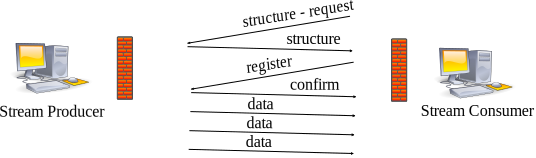
\includegraphics[width=0.8\columnwidth]{gsn-network-firewall}
  \caption{Experimental setup}
  \label{fig:gsn-network-firewall}
\end{figure}

In order to make the GSN to GSN communication more concrete, we provide more system level details below.
For using a remote virtual sensor, the first step is locating the \emph{contact point} of the GSN server which
hosts the prospective virtual sensor. By default, the contact point is \texttt{http://ip-address:gsn-port/gsn-handler}\footnote{The GSN port is specified in the \texttt{conf/gsn.xml} file and will be 22001 unless changed.}\footnote{In the \texttt{webapp/WEB-INF/web.xml} file, the GSN's RPC handler (the \texttt{gsn.GSNRPC} class) is mapped to \texttt{/gsn-handler}. One shouldn't confuse the \texttt{/gsn-handler} with \texttt{/gsn} which is designed to be used solely by the web/ajax interface and does not involved in XML-RPC calls.}.
If  the contact point is correctly identified, the response to a plain HTTP POST request 
returns a XML output.\footnote{The actual output represents an error as the request is not properly formatted.}\footnote{For sending plain HTTP POST requests
to \texttt{http://ip-address:gsn-port/gsn-handler}, you may want to use \url{http://code.google.com/p/rest-client/}. }

Correct identification of the contact point is crucial in success of using the remote virtual sensor.
Once the contact points identified successfully, one can define a stream which consume data from the other data source.
Note that consuming data from a remote virtual sensor doesn't require any kind of modifications at the remote host and in fact 
due to GSN's decoupled architecture, the remote virtual sensor is not even aware of its data consumers. In figure \ref{gsn2gsn-simple-figure},
the virtual sensor \texttt{ConsumerVS} running at the GSN server with the IP address of \texttt{3.3.3.3} under the port \texttt{22001} is interested
in getting data from the \texttt{CoolVS} running at the GSN server with the IP address of \texttt{4.4.4.4} under the port \texttt{22001}. To enable this
communication one has to use a source configuration similar to the one in figure \ref{gsn2gsn-simple-figure}.


\begin{figure}%[htb]
  \centering
  
\includegraphics[width=0.8\columnwidth]{gsn-comm-no-firewall}
  \caption{Simple GSN to GSN communication}
  \label{gsn2gsn-simple-figure}
\end{figure}


%\begin{figure}%[htb]
% \centering
%  \lstset{numbers=left, numberstyle=\footnotesize}
%\begin{lstlisting}
\begin{xmlcode}[caption={Source configuration for simple GSN to GSN communication.}, label=gsn2gsn-simple]
<address wrapper="remote">
  <predicate key="name">CoolVS</predicate>
  <predicate key="host">4.4.4.4</predicate>
  <predicate key="port">22001</predicate>
</address>        
\end{xmlcode}
%  \caption{Source configuration for simple GSN to GSN communication.}
%  \label{gsn2gsn-simple}
%\end{figure}

In some deployments, GSN servers are hosted behind a NAT an apache web server\footnote{The instruction for using GSN behind a apache web server is provided in appendix \todo{ref{app:gsn-apache}}.} which can cause port and/or IP change. This can be true for both the GSN data stream consumer and GSN data stream producer.
In these cases, one can use the more advanced form of the remote wrapper. Figure \ref{gsn2gsn-nat-figure} presents a sample setup in which both of the GSN data stream
consumer and data producer are behind firewall. The firewall at the consumer side has mapped \texttt{3.3.3.3:22001} into \texttt{1.1.1.1:82} and at the stream producer side
firewall has mapped \texttt{4.4.4.4:22001} into \texttt{2.2.2.2:80}.  To enable this kind of
communication one has to use a source configuration similar to the one in figure \ref{gsn2gsn-nat-figure}.


\begin{figure}%[htb]
  \centering
  \includegraphics[width=0.8\columnwidth]{gsn-comm-firewall}
  \caption{GSN to GSN communication with NAT}
  \label{gsn2gsn-nat-figure}
\end{figure}

%\begin{figure}%[htb]
%  \centering
%  \lstset{numbers=left, numberstyle=\footnotesize,basicstyle=\small}
%\begin{lstlisting}
\begin{xmlcode}[caption={Source configuration for NATed GSN to GSN communication.}, label=listing:xml:nat_remote_vsd]
<address wrapper="remote">
  <predicate key="name">CoolVS</predicate>
  <predicate key="local-contact-point">http://1.1.1.1:82/gsn-2</predicate>
  <predicate key="remote-contact-point">http://2.2.2.2:80/gsn-server</predicate>
</address>        
\end{xmlcode}
%  \caption{Source configuration for NATed GSN to GSN communication.}
%  \label{gsn2gsn-nat}
%\end{figure}

\subsection{\texttt{local} wrapper}
The \verb|local| wrapper is special version of \texttt{remote} wrapper (host = ``\texttt{127.0.0.1}'') which is optimized
for communication among two different virtual sensors inside the same GSN server. By having the
\texttt{local} wrapper optimized, we imply that most of the overhead associated with TCP/IP networking
calls are eliminated by using internal GSN calls instead. The \texttt{local} wrapper is recommend whenever
the end to end delay between two virtual sensors is important. In GSN, we have implemented the 
notification system so that the GSN server always gives priority to the local virtual sensors when it wans to disseminate
the stream elements thus the local virtual sensors usually get notified earlier.


\section{GSN Notifications}

\subsubsection{Introduction}

In GSN, virtual sensors can be configured to notify users of certain events, e.g. to send an Email notification to an user informing them that a particular event has occurred. To implement notifications in GSN is very straight forward. The basic principle is that once the virtual sensor query is answered as specified in the virtual sensor description file, e.g.

\begin{xmlcode}
<query>SELECT temperature FROM s1 WHERE temperature >= 100</query>
\end{xmlcode}

a notification can be triggered  by the java processing class

\begin{xmlcode}
<class-name>gsn.vsensor.EmailVirtualSensor</class-name>
\end{xmlcode}

see examples in next section. Thus, any type of notifications, e.g. Email, SMS, SIP, Fax, MMS can be implemented easily in a virtual sensor processing class. 

The technical details of implementing notifications are left to the designer. Below are three examples of some of the notification services already implemented in GSN.

\section{Notes}


\subsubsection{Where is the DTD for the virtual sensor?}
We are using JiBX Java-XML binding project. The structure of the virtual sensor descriptor file is defined in \texttt{conf/VirtualSensorDescription.xml}.

Have a look to the \chapref{quickref_vsd_dtd}.

\subsubsection{Which databases we support ?}
At the moment we are supporting HSqlDB and MySQL. Checkout the mailing list for the latest issues regarding the other databases and their
support status.
\subsubsection{Which projects are using GSN ?}
There are over 10 EU/Swiss funding research projects using GSN as their core technology.
\subsubsection{GSN.XML file}
\subsection{GeoRSS}
\subsection{Network communication}
Looking inside the GSN infrastructure, there are at least half a dozen difference network communication channels are used. In this section I would like to dive in to the details
of the some major communication protocols designed and implemented in GSN. 

\subsubsection{Reusing Data Streams}

One of the main ideas behind the virtual sensors is resuability. The resuability comes in two forms.
First being able to recreate the same processing logic on different data streams.
Second being able to reuse streaming data produced by other parties over the internet and possibly create a new data stream but instrumenting the original streams.
In this section, I present the both high level and low level details associated with the second aspect of the reusability.

The virtual sensor descriptor file is the first place which specifies the intention of reusing streaming data from another virtual sensor. The source virtual sensor can be located
anywhere as long as it is accessible through the network, this ofcourse includes the local machine and any other machine on the Internet. 


In GSN, our vision is having an internet scale streaming world in which people can publish streaming data which
can be produced directly using some sort of a measurement device which can range from a physical wireless sensor to stock ticks from a financial market.








	% Images index
	\listoffigures
	% Tables index
	\listoftables	
	% Listings index
	\lstlistoflistings
	% Bibliography
	\bibliographystyle{plain} % abbrv, plain, alpha
	\bibliography{references}
	%
	\appendix
	\graphicspath{{chapters/ch-quickref/figures/}}

\chapter{Quick Reference Guide}

\section{Virtual Sensors (\vs)}

%
% Virtual Sensors
%
\subsection{\vsd DTD \label{quickref_vsd_dtd}}

All the \vs are configured with an XML Virtual Sensor Description file (\vsd).
A graphical representation of the \vsd Document Type Definition (DTD) is available on the \figref{figure:vsd_dtd}. The description of all these tags are given in the
\tableref{table:vsd_dtd}.

\image{vs-quick-ref-marked.pdf}{1.0}{90}{\vsd DTD Quick Reference Card}{figure:vsd_dtd}

\begin{table*}[!htp]
	\centering
	{\normalfont\footnotesize
	\begin{tabulary}{\textwidth}{|C|J|C|J|J|}%
	\hline
		\multicolumn{5}{|c|}{\textbf{VSD DTD Quick Reference Card Description}} \\
	\hline
	\hline
		\textbf{Tag} &
		\textbf{Name} &
		\textbf{Mandatory} &
		\textbf{Allowed Values} &
		\textbf{Description} \\
	\hline
	\hline
		1 & name & 1 only & alpha&Identifies the VS and must be unique in an instance of GSN \\ \hline
		2 & protected & 0 or 1 & \todo{TODO} &\todo{TODO}  \\ \hline
		4 & publish-to-microsoft-research-map & 0 or 1 & & \\ \hline
		5 & processing-class & \todo{?} & & Container for \vsp specification   \\ \hline
		6 & class-name  & 1 only & \todo{TODO} & Path to Java implementation of \vsp   \\ \hline
		7 - 10 & init-params & 0 or 1 &\todo{TODO} & Parameter specific to \vsp (Refer to section \ref{sec:quickref_vsp})  \\ \hline
		11 & unique-timestamps & 0 or 1 &\todo{TODO} &\todo{TODO}  \\ \hline
		12 & output-structure & 1 only &\todo{TODO} &\todo{TODO}  \\ \hline
		13 & field & 0 or more &\todo{TODO} &\todo{TODO}  \\ \hline
		14 & name & 1 per field &\todo{TODO}  &\todo{TODO}  \\ \hline
		15 & type & 1 per field &\todo{TODO} &\todo{TODO}  \\ \hline
		16 & description & 1 per field & Free text & Description of output item  \\ \hline
		17 & output-specification & 0 or 1 &\todo{TODO} &\todo{TODO}  \\ \hline
		18 & rate & 1 only &\todo{TODO} &\todo{TODO}  \\ \hline
		19 & web-input & 0 or 1 &\todo{TODO} &\todo{TODO}  \\ \hline
		20 & password & 0 or 1 &\todo{TODO} &\todo{TODO}  \\ \hline
		21 & command & 0 or more &\todo{TODO} &\todo{TODO}  \\ \hline
		22 & name &  1 only  &\todo{TODO} &\todo{TODO}  \\ \hline
		23 & field & 0 or more &\todo{TODO} &\todo{TODO}  \\ \hline
		24 & name & 1 only &\todo{TODO} &\todo{TODO}  \\ \hline
		25 & type & 1 only &\todo{TODO} &\todo{TODO}  \\ \hline
		26 & description & 1 only &\todo{TODO} & Field description  \\ \hline
		27 & description & 0 or 1 &\todo{TODO} & \vs Description   \\ \hline
		28 & life-cycle & 0 or 1 &\todo{TODO} &\todo{TODO}  \\ \hline
		29 & pool-size & 1 only &\todo{TODO} &\todo{TODO}  \\ \hline
		30 & addressing & 1 only &\todo{TODO} &\todo{TODO}  \\ \hline
		31 & predicate & 0 or more &\todo{TODO} &\todo{TODO}  \\ \hline
		32 & key &\ 1 only &\todo{TODO} &\todo{TODO}  \\ \hline
		33 & value & 1 only &\todo{TODO} &\todo{TODO}  \\ \hline
		34 & storage & 1 only &\todo{TODO} &\todo{TODO}  \\ \hline
		35 & history-size & 1 only &\todo{TODO} &\todo{TODO}  \\ \hline
		36 & streams & 1 only &\todo{TODO} &\todo{TODO}  \\ \hline
		37 & stream & 0 or more &\todo{TODO} &\todo{TODO}  \\ \hline
		38 & name & 1 only &\todo{TODO} &\todo{TODO}  \\ \hline
		39 & count & 0 or 1 &\todo{TODO} & deprecated ?\\ \hline
		40 & rate & 1 only &\todo{TODO} &\todo{TODO}  \\ \hline
		41 & source & 0 or more &\todo{TODO} &\todo{TODO}  \\ \hline
		42 & alias{TODO} & 1 only &\todo{TODO} &\todo{TODO}  \\ \hline
		43 & disconnect-buffer-size & 0 or 1 &\todo{TODO} &\todo{TODO}  \\ \hline
		44 & storage-size & 0 or 1 &\todo{TODO} &\todo{TODO}  \\ \hline
		45 & slide & 0 or 1 &\todo{TODO} &\todo{TODO}  \\ \hline
		46 & sampling-rate & 0 or 1 &\todo{TODO} &\todo{TODO}  \\ \hline
		47 & address & 0 or 1 &\todo{TODO} &\todo{TODO}  \\ \hline
		48 & wrapper & 1 or more &\todo{TODO} &\todo{TODO}  \\ \hline
		49 - 51 & predicate & 0 or more &\todo{TODO} & Predicates are specific to wrappers (Refer to section \ref{sec:quickref_wrappers})  \\ \hline
		52 & query (source) & 1 only &\todo{TODO} &\todo{TODO}  \\ \hline
		53 & query (stream) & 1 only&\todo{TODO} &\todo{TODO}  \\ \hline
	\end{tabulary}
	}
	\caption{\vsd DTD Quick Reference Card Description}
	\label{table:vsd_dtd}
\end{table*}
\newpage
\subsection{Email Notification \vs \label{quickref_email_notification_vs}}

This virtual sensor implements an Email notification system for \gsn. 
This \vs is based on the \chapref{email:vsp} \vsp and the \chapref{multiformat:wrapper} \wrapper.
The \listingref{listing:xml:emailnotification_vsd} shows an example of \vsd for this \vs.

\begin{xmlcode}[caption={Sample of Email Notification VSD file}, label=listing:xml:emailnotification_vsd]
<virtual-sensor name="email" priority="10">
	<processing-class>
		<class-name>gsn.vsensor.EmailVirtualSensor</class-name>
		<init-params>
			<param name="RECEIVER">John Connor</param>
			<param name="receiver-email">john.connor@gmail.com</param>
			<param name="sender-email">admin@sensorinternet.com</param>
			<param name="mail-server">smtp.gmail.com</param>
			<param name="subject">Abnormal Temperature Detected</param>
			<param name="MESSAGE">Sensor 114 has a value of 100 C.</param>   
		</init-params>
		<output-structure>
			<field name="temp" type="double" />
		</output-structure>
	</processing-class>
	<description>Send an Email Notification</description>
	<life-cycle pool-size="10" />
	<addressing />
	<storage history-size="10m" />
	<streams>
		<stream name="in1">
			<source alias="s1" sampling-rate="1" storage-size="1">
				<address wrapper="multiformat">
					<predicate key="HOST">localhost</predicate>
					<predicate key="PORT">22001</predicate>
				</address>
				<query>SELECT * FROM wrapper</query>
			</source>
			<query>SELECT temperature FROM s1 WHERE temperature >= 100</query>
		</stream>
	</streams>
</virtual-sensor>
\end{xmlcode}


\newpage
\subsection{SMS Notification \vs \label{sms:vsp}}

This virtual sensor implements SMS (Short Message Service) notification. This virtual sensor is very similar to the email virtual sensor – an email is sent to a Mobile phone operator or SMS gateway provider based on the user's mobile account and the email is converted and send as a SMS to the given phone number.
This \vs is based on the \chapref{sms:vsp} \vsp and the \chapref{multiformat:wrapper} \wrapper.
The \listingref{listing:xml:smsnotification_vsd} shows an example of \vsd for this \vs.

\begin{xmlcode}[caption={Sample of SMS Notification VSD file}, label=listing:xml:smsnotification_vsd]
<virtual-sensor name="sms" priority="10">
	<processing-class>
		<class-name>gsn.vsensor.SMSVirtualSensor</class-name>
		<init-params>
			<param name="phone-number">004413243545</param>
			<param name="password">3524</param>
			<param name="sms-server">vodafone.co.uk</param>
			<param name="message-format">Temperature: $TEMP$</param>
		</init-params>
		<output-structure>
			<field name="temp" type="double" />
		</output-structure>
	</processing-class>
	<description>Send a SMS Notification</description>
	<life-cycle pool-size="10" />
	<addressing />
	<storage history-size="10m" />
	<streams>
		<stream name="in1">
			<source alias="s1" sampling-rate="1" storage-size="1">
				<address wrapper="multiformat">
					<predicate key="HOST">localhost</predicate>
					<predicate key="PORT">22001</predicate>
				</address>
				<query>SELECT * FROM wrapper</query>
			</source>
			<query>SELECT temperature FROM s1 WHERE temperature >= 100</query>
		</stream>
	</streams>
</virtual-sensor>
\end{xmlcode}

Note that this virtual sensor will only work if you have an account with a mobile phone operator or an internet SMS gateway provider. 
\newpage
\subsection{Voip Notification \vs \label{voip:vsp}}

This virtual sensor implements a phone call notification. The virtual sensor makes a phone call when a condition 
in the virtual sensor query is triggered. The virtual sensor is configured to work with Asterisk\footnote{\url{http://www.asterisk.org/}}. So, you will need to install\footnote{\url{http://www.trixbox.org/downloads}} or have an existing asterisk server running. To configure the sensor with asterisk you will need to add the following line: \textit{``\#include extensions\_gsn.conf''} to the \textit{extensions\_custom.conf} file in asterisk (/etc/asterisk/extensions\_custom.conf). Once the virtual sensor is deployed, it automatically creates a dial plan in asterisk and registers extensions needed to make the phone calls, minimal configuration is required.
This will include the any extensions created by the virtual sensor in the file \textit{extensions\_gsn.conf}. Depending on the number of times the virtual sensor is deployed, an extension with the virtual sensor name and a random extension number (internal to asterisk) will be created.
The virtual sensor uses the Manager API to connect (login) to asterisk and execute remote commands (e.g. load dial plan, make phone call, call forward). To loging to the asterisk manager, you have to create an account and add your IP address in the \textit{manager.conf} file in asterisk (/etc/asterisk/manager.conf):

\begin{bashcode}[caption={Settings for Manager.conf file in Asterisk}, label=listing:bash:voip_vsd]
[testuser]
secret = mypassword
permit=192.168.12.101/255.255.0.0
read = system,call,log,verbose,command,agent,user
write = system,call,log,verbose,command,agent,user
\end{bashcode}

Where, \textit{testuser} is the username and \textit{secret} is the password. In \textit{permit} add your IP address (otherwise asterisk will block you). As part of asterisk, you will also need to install the \textit{festival} text to speech system\footnote{\url{http://www.cstr.ed.ac.uk/projects/festival/}} and the \textit{sox} utility\footnote{\url{http://sox.sourceforge.net/}}. These programs are used by the virtual sensor to convert the notification message (string) to speech (audio) to be played by asterisk. If using linux/ubuntu, do an  \textit{``apt-get install festival sox''}.

This \vs is based on the \chapref{voip:vsp} \vsp and the \chapref{multiformat:wrapper} \wrapper.
The \listingref{listing:xml:voip_vsd} shows an example of \vsd for this \vs.

\begin{xmlcode}[caption={Sample of VoIP VSD file}, label=listing:xml:voip_vsd]
<virtual-sensor name="phone" priority="10">
	<processing-class>
	<class-name>gsn.vsensor.VoipVirtualSensor</class-name>
		<init-params>
			<param name="username">testuser</param>
			<param name="password">mypassword</param>
			<param name="host">asterisk-server.com</param>
			<param name="number">0041786831809</param>
			<param name="message">The temperature in the lab is too high.</param>
		</init-params>
		<output-structure>
			<field name="temperature" type="double" />
		</output-structure>
	</processing-class>
	<description>Makes a phone call when a query in the virtual sensor is satisfied.</description>
	<life-cycle pool-size="10" />
	<addressing>
		<predicate key=""></predicate>
	</addressing>
	<storage history-size="1h" />
  <streams>
    <stream name="input1">
    <source alias="source1" sampling-rate="1" storage-size="1">
      <address wrapper="multiformat">
          <predicate key="HOST">localhost</predicate>
          <predicate key="PORT">22001</predicate>
      </address>
      <query>SELECT temperature, timed FROM wrapper WHERE packet_type=2</query>
    </source>
    <query>SELECT temperature, timed FROM source1</query>
    </stream> 
  </streams>
</virtual-sensor>
\end{xmlcode}

Note that this virtual sensor will only work if you have an account with a mobile phone operator or an internet SMS gateway provider. 
\newpage
\subsection{R \vs \label{r:vsp}}
The software architecture of GSN allows the integration of third-party numerical packages such as Matlab, Mathematica, and more recently the R statistical package. In this section, we describe how to integrate and perform data analysis using R and GSN. 

\subsubsection{Installation and Setup}
R is a programming language and a software package for statistical computing and analysis. R provides a range of techniques for statistical analysis such as liner and nonlinear modeling, classical statistical test, time-series analysis. The R software platform is composed of an engine that can interpret and execute R scripts or programs (in a similar way to GNU Octave or Matlab). The R engine can be invoked from the console or over the network using a TCP/IP server called Rserve. In this section, we describe how to configure the R and the Rserve server.

\subsubsection*{Installation}
First, we have to install R. R is available in several platforms, depending on your platform you will have to follow specific instructions. We recommend to read the documentation from the official project website: \url{http://www.r-project.org/}. 

\subsubsection*{Rserve TCP/IP Server}
Rserve is a TCP/IP server which allows other programs to use invoke R from various languages without the need to initialize R or link against R library. Rserve can be downloaded from the following website: \url{http://www.rforge.net/Rserve/}. Rserve is written in Java and it has bindings for other languages.
Rserve comes as a R package, therefore, to install and run Rserve, the library and the package have to be invoked within R as follows:

\begin{bashcode}[caption={Running R and starting Rserve server.}, label=listing:bash:r_vsd]
user@host\# R
R version 2.6.2 (2008-02-08) 
Copyright (C) 2008 The R Foundation for Statistical Computing 

> library(Rserve) 
> Rserve()
\end{bashcode}

This will load the Rserve library and start the Rserve TCP/IP server on the localhost. The default port is 6311. To read more about how to invoke R using Rserve, please refer to the Rserve documentation website: \url{http://www.rforge.net/Rserve/}.

This \vs is based on the \chapref{voip:vsp} \vsp and the \chapref{multiformat:wrapper} \wrapper.
The \listingref{listing:xml:r_vsd} shows an example of \vsd for this \vs.

\begin{xmlcode}[caption={Sample of R VSD file}, label=listing:xml:voip_vsd]
<virtual-sensor name="plot" priority="10">
	<processing-class>
	<class-name>gsn.vsensor.RVirtualSensor</class-name>
		<init-params>
      <param name="plot">2D</param>
			<param name="device">jpeg</param>
			<param name="operation">x<-rnorm(10);plot(x,$temperature$);</param>
		</init-params>
		<output-structure>
			<field name="plot" type="binary:image/jpeg"/>
		</output-structure>
	</processing-class>
	<description>Plots a graph using R.</description>
	<life-cycle pool-size="10"/>
	<addressing>
		<predicate key=""></predicate>
	</addressing>
	<storage history-size="1h"/>
  <streams>
    <stream name="input1">
    <source alias="source1" sampling-rate="1" storage-size="1">
      <address wrapper="multiformat">
          <predicate key="HOST">localhost</predicate>
          <predicate key="PORT">22001</predicate>
      </address>
      <query>SELECT temperature, timed FROM wrapper WHERE packet_type=2</query>
    </source>
    <query>SELECT temperature, timed FROM source1</query>
    </stream> 
  </streams>
</virtual-sensor>
\end{xmlcode}

\newpage
\subsection{GPS \vs \label{quickref_tinyos_vs}}

This virtual sensor integrates Generic NMEA GPS Devices with \gsn.
This \vs is based on the \chapref{bridge:vsp} \vsp and the \chapref{gpsd:wrapper} \wrapper.
The \listingref{listing:xml:gpsd_vsd} shows an example of \vsd for this \vs.

\begin{xmlcode}[caption={Sample of VSD using the Gpsd Wrapper}, label=listing:xml:gpsd_vsd]
<virtual-sensor name="gpsd" priority="10">
	<processing-class>
		<class-name>gsn.vsensor.BridgeVirtualSensor</class-name>
		<init-params/>
		<output-structure>
			<field name="Latitude" type="double"/>
			<field name="Longitude" type="double"/>
			<field name="Altitude" type="double"/>
			<field name="RateOfClimb" type="double"/>
			<field name="SpeedOverGround" type="double"/>
			<field name="GpsDeviceName" type="char(255)"/>
			<field name="GpsProtocol" type="char(255)"/>
			<field name="CountOfSatellites" type="int"/>
			<field name="VerticalDOP" type="double"/>
			<field name="HorizontalDOP" type="double"/>
			<field name="PositionalDOP" type="double"/>
			<field name="TimeDOP" type="double"/>
			<field name="GeometricDOP" type="double"/>
		</output-structure>
	</processing-class>
	<description>Send a SMS Notification</description>
	<life-cycle pool-size="10" />
	<addressing />
	<storage history-size="10m" />
	<streams>
		<stream name="input1">
			<source alias="source1" sampling-rate="1" storage-size="1">
				<address wrapper="gpsd">
					<predicate key="ListenerPort">2947</predicate>
					<predicate key="SamplingRate">2000</predicate>
					<predicate key="Timeout">22000</predicate>
				</address>
				<query>select * from wrapper</query>
			</source>
			<query>select * from source1</query>
		</stream> 
	</streams>
</virtual-sensor>
\end{xmlcode}
\newpage
\subsection{TinyOS \vs \label{quickref_tinyos_vs}}

This virtual sensor integrates TinyOS\footnote{\url{http://www.tinyos.net/}} data sources with \gsn.
This \vs is based on the \chapref{bridge:vsp} \vsp and the \chapref{tinyos-mig:wrapper} \wrapper.
The \listingref{listing:xml:tinyos_vsd} shows an example of \vsd for this \vs.

\begin{xmlcode}[caption={Sample of VSD}, label=listing:xml:tinyos_vsd]
<virtual-sensor name="ss_migwrapper" priority="10" >
    <processing-class>
       <class-name>gsn.vsensor.BridgeVirtualSensor</class-name>
       <unique-timestamps>true</unique-timestamps>
        <output-structure>
			<field name="SYSVOLTAGE" type="INTEGER" />
			<field name="REALSYSVOLTAGE_V" type="DOUBLE" />
			<field name="SDIVOLTAGE" type="INTEGER" />
			<field name="REALSDIVOLTAGE_V" type="DOUBLE" />
			<field name="TEMPERATURE" type="INTEGER" />
			<field name="REALTEMPERATURE_C" type="DOUBLE" />
			<field name="MOISTURE" type="INTEGER" />
			<field name="APPROXMOISTURE_REL" type="DOUBLE" />
			<field name="REALMOISTURE_REL" type="DOUBLE" />
			<field name="TIMESTAMP" type="BIGINT" />
       </output-structure>
    </processing-class>
    <description> TODO Add a description</description>
    <life-cycle pool-size="10" />
    <addressing/>
    <storage />
    <streams>
    <stream name="data">
      <source alias="source" storage-size="1" sampling-rate="1">
        <address wrapper="ss_tinyos-mig">
           		<predicate key="ss-host">localhost</predicate>
          		<predicate key="ss-port">25000</predicate>
          		<predicate key="continue-on-error">true</predicate>
          		<predicate key="wrapper-name">mig2</predicate>
          		<predicate key="wrapper-keep-processed-ss-entries">false</predicate>
               <predicate key="source">sf@permafrozer.ethz.ch:9001</predicate>
               <predicate key="message-classname">ch.ethz.permafrozer.DozerDataMsg</predicate>
               <predicate key="message-length">23</predicate>
               <predicate key="getter-prefix">get</predicate>
           </address>
        <query> select * from wrapper </query>
      </source>
      <query> select * from source</query>
    </stream>
  </streams>
</virtual-sensor>
\end{xmlcode}

%
% Virtual Sensors Processing classes
%
\newpage
\section{Virtual Sensor Processing classes (\vsp) \label{sec:quickref_vsp}}
\subsection{gsn.vsensor.EmailVirtualSensor \vsp \label{email:vsp}}

\begin{table*}[!htp]
	\centering
	{\normalfont\footnotesize
	\begin{tabulary}{\textwidth}{|C|C|C|C|J|}%
	\hline
		\multicolumn{5}{|c|}{\textbf{Parameters for gsn.vsensor.EmailVirtualSensor \vsp}} \\
	\hline
	\hline
		\textbf{Parameter Name} &
		\textbf{Type} &
		\textbf{Mandatory} &
		\textbf{Default} &
		\textbf{Description} \\
	\hline
	\hline
		RECEIVER &
		String &	
		Yes &
		None &
		Name of the email recipient \\
	\hline
		receiver-email &
		String &	
		Yes &
		None &	
		Email address of the recipient \\
	\hline
		sender-email &
		String &	
		Yes &
		None &	
		Email address of the sender \\
	\hline
		mail-server &
		String &	
		Yes &
		None &	
		URL for the email (SMTP) server \\
	\hline
		subject &
		String &	
		Yes &
		None &	
		Subject of the email \\
	\hline
		message &
		String &	
		Yes &
		None &	
		Email message \\
	\hline
	\end{tabulary}
	}
	\caption{Parameters for gsn.vsensor.EmailVirtualSensor \vsp}
	\label{table:parameters_email_vsp}
\end{table*}
\input{chapters/ch-quickref/vsp/sms_vsp}
\subsection{gsn.vsensor.VoipVirtualSensor \vsp}

\begin{table*}[!htp]
	\centering
	{\normalfont\footnotesize
	\begin{tabulary}{\textwidth}{|C|C|C|C|J|}%
	\hline
		\multicolumn{5}{|c|}{\textbf{Parameters for gsn.vsensor.VoipVirtualSensor \vsp}} \\
	\hline
	\hline
		\textbf{Parameter Name} &
		\textbf{Type} &
		\textbf{Mandatory} &
		\textbf{Default} &
		\textbf{Description} \\
	\hline
	\hline
		username &
		String &	
		Yes &
		None &
		Username to login to the asterisk server. \\
	\hline
		password &
		String &
		Yes &
		None &
		Password to login to the asterisk server. \\
	\hline
		host &
		String &
		Yes &
		None &
		DNS address of the asterisk server. \\
	\hline
		number &
		String &
		Yes &
		None &
		Telephone number to dial. \\
	\hline
    message &
    String &
    Yes &
    None &
    Notification message. \\
  \hline
	\end{tabulary}
	}
	\caption{Parameters for gsn.vsensor.VoipVirtualSensor \vsp \label{table:parameters_voip_vsp}}
	
\end{table*}

\subsection{gsn.vsensor.RVirtualSensor \vsp}

\begin{table*}[!htp]
	\centering
	{\normalfont\footnotesize
	\begin{tabulary}{\textwidth}{|C|C|C|C|J|}%
	\hline
		\multicolumn{5}{|c|}{\textbf{Parameters for gsn.vsensor.RVirtualSensor \vsp}} \\
	\hline
	\hline
		\textbf{Parameter Name} &
		\textbf{Type} &
		\textbf{Mandatory} &
		\textbf{Default} &
		\textbf{Description} \\
	\hline
	\hline
		phone-number &
		String &	
		Yes &
		None &
		The mobile phone number to send the message \\
	\hline
		password &
		String &
		Yes &
		None &
		The password to login to the mobile operator or SMS gateway provider \\
	\hline
		sms-server &
		String &
		Yes &
		None &
		URL address of the mobile phone operator or SMS gatewat provider \\
	\hline
		message-format &
		String &
		Yes &
		None &
		The format of the SMS message in StringTemplate-syntax, e.g. Temperature: \$TEMP\$ where TEMP has some value given from the GSN StreamElement \\
	\hline
	\end{tabulary}
	}
	\caption{Parameters for gsn.vsensor.RVirtualSensor \vsp \label{table:parameters_r_vsp}}
	
\end{table*}

\subsection{gsn.vsensor.BridgeVirtualSensor \vsp \label{bridge:vsp}}

\begin{table*}[!htp]
	\centering
	{\normalfont\footnotesize
	\begin{tabulary}{\textwidth}{|C|C|C|C|J|}%
	\hline
		\multicolumn{5}{|c|}{\textbf{Parameters for gsn.vsensor.BridgeVirtualSensor \vsp}} \\
	\hline
	\hline
		\textbf{Parameter Name} &
		\textbf{Type} &
		\textbf{Mandatory} &
		\textbf{Default} &
		\textbf{Description} \\
	\hline
	\hline
		\todo{TODO} &
		\todo{TODO} &	
		\todo{TODO} &
		\todo{TODO} &
		\todo{TODO} \\
	\hline
	\end{tabulary}
	}
	\caption{Parameters for gsn.vsensor.BridgeVirtualSensor \vsp}
	\label{table:parameters_bridge_vsp}
\end{table*}

%
% Wrappers
%
\newpage
\section{Wrappers \label{sec:quickref_wrappers}}
\subsection{Safe Storage Wrappers Default parameters}

The parameters shown on the \listingref{table:safe_storage_parameters} must be added to each \wrapper that support the 
Safe Storage feature. An example of \wrapper that use this feature is described in \chapref{tinyos-mig:wrapper}.

\begin{table*}[!htp]
	\centering
	{\normalfont\footnotesize
	\begin{tabulary}{\textwidth}{|C|C|C|C|J|}%
	\hline
		\multicolumn{5}{|c|}{\textbf{Safe Storage Parameters}} \\
	\hline
	\hline
		\textbf{Parameter Name} &
		\textbf{Type} &
		\textbf{Mandatory} &
		\textbf{Default} &
		\textbf{Description} \\
	\hline
	\hline
		ss-host &
		String &	
		Yes &
		None &
		The machine host name that runs the Safe Storage \\
	\hline
		ss-port &
		Integer &	
		Yes &
		None &
		The server port on which Safe Storage listen for connections \\
	\hline
		wrapper-name &
		String &	
		Yes &
		None &
		The Safe Storage side wrapper full classname (must extends \inlinecode{gsn.acquisition2.wrappers.AbstractWrapper2}) 
		or the short name from the \path{conf/safe\_storage\_wrappers.properties} file. \\
	\hline
		wrapper-keep-processed-ss-entries &
		Boolean &
		No &
		true &
		If this option is set to \inlinecode{true}, all the entries (processed or not) kept into the Safe Storage storage.
		If this option is set to \inlinecode{false}, the processed entries are removed from the Safe Storage storage once processed. \\
	\hline
		continue-on-error &
		Boolean &	
		No &
		true &
		Not yet implemented \\
	\hline
	\end{tabulary}
	}
	\caption{Safe Storage Parameters}
	\label{table:safe_storage_parameters}
\end{table*}
\subsection{multiformat \wrapper \label{multiformat:wrapper}}

\begin{table*}[!htp]
	\centering
	{\normalfont\footnotesize
	\begin{tabulary}{\textwidth}{|C|C|C|C|J|}%
	\hline
		\multicolumn{5}{|c|}{\textbf{multiformat \wrapper Parameters}} \\
	\hline
	\hline
		\textbf{Parameter Name} &
		\textbf{Type} &
		\textbf{Mandatory} &
		\textbf{Default} &
		\textbf{Description} \\
	\hline
	\hline
		\todo{TODO} &
		\todo{TODO} &	
		\todo{TODO} &
		\todo{TODO} &
		\todo{TODO} \\

	\hline
	\hline
		\multicolumn{2}{|l}{Support Safe Storage} &
		\multicolumn{3}{l|}{No} \\
		\multicolumn{2}{|l}{GSN \wrapper Classname} &
		\multicolumn{3}{l|}{gsn.wrappers.MultiFormatWrapper (multiformat)} \\
	\hline
	\end{tabulary}
	}
	\caption{multiformat \wrapper Parameters}
	\label{table:multiformat_wrapper_parameters}
\end{table*}


\begin{table*}[!htp]
	\centering
	{\normalfont\footnotesize
	\begin{tabulary}{\textwidth}{|C|C|J|}%
	\hline
		\multicolumn{3}{|c|}{\textbf{multiformat \wrapper Output Structure}} \\
	\hline
	\hline
		\textbf{Name} &
		\textbf{Type} &
		\textbf{Description} \\
	\hline
	\hline
		\todo{TODO} &
		\todo{TODO} &
		\todo{TODO} \\
	\hline 
	\end{tabulary}
	}
	\caption{multiformat \wrapper Output Structure}
	\label{table:multiformat_wrapper_output_structure}
\end{table*}
\subsection{ss\_tinyos-mig \wrapper \label{tinyos-mig:wrapper}}

The TinyOS \wrapper can receive data from both version 1.x and 2.x TinyOS based networks.
This \wrapper can interract with any TinyOS compatible Base Station and any type of TinyOS Packet Source.
For instance The TinyOS wrapper can interact with the serial forwarder (provided by TinyOS distribution) which 
inturn presents a sensor network. In order to use the TinyOS wrapper with a sensor network you need to first generate the java
representation of the message structures used in the network (in TinyOS they are defined in the \inlinecode{.h} files). 
NesC language provides a tool called \inlinecode{mig} (message
interface generator for nesC) for this purpose. The tool has a standard man page
documentation in addition to being described in the lession 4 of the TinyOS 2
tutorial
\footnote{Further informations can be found at\\ \url{http://www.tinyos.net/tinyos-1.x/doc/nesc/mig.html}\\ \url{http://www.tinyos.net/tinyos-2.x/doc/html/tutorial/lesson4.html}\\ \url{http://www.tinyos.net/tinyos-1.x/doc/tutorial/lesson6.html}}.

Both TinyOS 1.x and 2.x are using very same package structures and class names which generates conflict when 
you have both TinyOS1.x and 2.x jar files in your classpath (which is the case for \gsn).
To solve this issue, \gsn provides a slightly modified version of the TinyOS 1.x java tools by renaming the \inlinecode{net.tinyos.xxx} package to \inlinecode{net.tinyos1x.xxx}.
Thus the messages classes generated with MIG must be configured depending on the version of TinyOS your are using. The \tableref{table:tinyos_mig_version} shows the class that your
MIG generated messages must extend (directly or not directly).

\begin{table*}[!htp]
	\centering
	{\normalfont\footnotesize
	\begin{tabulary}{\textwidth}{|C|J|}%
	\hline
		\textbf{TinyOS version} &
		\textbf{Must extends} \\
	\hline
	\hline
		1.x &
		\inlinecode{net.tinyos1x.message.Message} \\
	\hline
		2.x &
		\inlinecode{net.tinyos.message.Message} \\
	\hline
	\end{tabulary}
	}
	\caption{Superclass for TinyOS messages classes}
	\label{table:tinyos_mig_version}
\end{table*}

\begin{table*}[!htp]
	\centering
	{\normalfont\footnotesize
	\begin{tabulary}{\textwidth}{|C|C|C|C|J|}%
	\hline
		\multicolumn{5}{|c|}{\textbf{ss\_tinyos-mig \wrapper Parameters}} \\
	\hline
	\hline
		\textbf{Parameter Name} &
		\textbf{Type} &
		\textbf{Mandatory} &
		\textbf{Default} &
		\textbf{Description} \\
	\hline
	\hline
		source &
		String &	
		Yes &
		None &
		The TinyOS data source \newline{}eg. \url{sf@serial.forwarder.url:9001}  \\
	\hline
		message-classname &
		String &
		Yes &
		None &
		The full package path to the message class generated by MIG\newline{}eg. \inlinecode{ch.ethz.permafrozer.DozerDataMsg} \\
	\hline 
		message-length &
		Integer &
		No &
		\inlinecode{DEFAULT\_MESSAGE\_SIZE} &
		Override the default size of the messages received \\
	\hline
		getter-prefix &
		String &
		No &
		get\_ &
		The methods of the message class that contain this prefix will be added in the output structure. 
		Keep the default value for the messages generated with MIG. \\
	\hline
	\hline
		\multicolumn{2}{|l}{Support Safe Storage} &
		\multicolumn{3}{l|}{Yes (Parameters listed on \tableref{table:safe_storage_parameters} must be added.)} \\
		\multicolumn{2}{|l}{SS \wrapper Classname} &
		\multicolumn{3}{l|}{gsn.acquisition2.wrappers.MigMessageWrapper2 (mig2)} \\
		\multicolumn{2}{|l}{GSN \wrapper Classname} &
		\multicolumn{3}{l|}{gsn.acquisition2.wrappers.MigMessageWrapperProcessor (ss\_tinyos-mig)} \\

	\hline
	\end{tabulary}
	}
	\caption{ss\_tinyos-mig \wrapper Parameters}
	\label{table:tinyos-mig_parameters}
\end{table*}

This \wrapper infers the output structure from the methods names contained into the MIG generated message class and the superclasses. To filter these methods, 
This \wrapper applies a prefix pattern matching on the methods names. The mapping between the TinyOS types and the types to use in your \vsd are shown on the 
\tableref{table:tinyos-mig_wrapper_output_structure}.

\begin{table*}[!htp]
	\centering
	{\normalfont\footnotesize
	\begin{tabulary}{\textwidth}{|C|C|C|J|}%
	\hline
		\multicolumn{4}{|c|}{\textbf{ss\_tinyos-mig \wrapper Output Structure}} \\
	\hline
	\hline
		\textbf{nesC} &
		\textbf{Java} &
		\textbf{\vsd} &
		\textbf{Description} \\
	\hline
	\hline
		nx\_int8\_t &
		byte &
		TINYINT &
		8-bit signed \\
	\hline 
		nx\_uint8\_t &
		short &
		SMALLINT &
		8-bit unsigned \\
	\hline 
		nx\_int16\_t &
		short &
		SMALLINT &
		16-bit signed \\
	\hline 
		nx\_uint16\_t &
		int &
		INTEGER &
		16-bit unsigned \\
	\hline 
		nx\_int32\_t &
		int &
		INTEGER &
		32-bit signed \\
	\hline 
		nx\_uint32\_t &
		long &
		BIGINT &
		32-bit unsigned \\
	\hline 
		NOT SUPPORTED &
		float &
		DOUBLE &
		32-bit floating point number \\
	\hline 
		NOT SUPPORTED &
		double &
		DOUBLE &
		64-bit floating point number \\
	\hline 
	\hline 
		\multicolumn{4}{|c|}{Arrays of the listed types are also supported.} \\
	\hline 
	\end{tabulary}
	}
	\caption{ss\_tinyos-mig \wrapper Output Structure}
	\label{table:tinyos-mig_wrapper_output_structure}
\end{table*}

\subsection{\todo{GpsdWrapper} \wrapper \label{gpsd:wrapper}} 

GpsdWrapper is a GSN wrapper for communicating with gpsd and supports querying GPS devices compliant to

\begin{itemize}
 \item NMEA 0183 protocol
 \item Rockwell binary protocol
 \item TSIP binary protocol
 \item SiRF protocol
 \item Garmin binary protocol
 \item Evermore binary protocol
\end{itemize}

\todo{Where are the source files?}

\begin{table*}[!htp]
	\centering
	{\normalfont\footnotesize
	\begin{tabulary}{\textwidth}{|C|C|C|C|J|}%
	\hline
		\multicolumn{5}{|c|}{\textbf{\todo{GpsdWrapper} \wrapper Parameters}} \\
	\hline
	\hline
		\textbf{Parameter Name} &
		\textbf{Type} &
		\textbf{Mandatory} &
		\textbf{Default} &
		\textbf{Description} \\
	\hline
	\hline
		HostName &
		String &	
		No &
		localhost &
		The hostname of GPS Daemon \\
	\hline
		ListenerPort &
		Integer &
		No &
		2947 &
		The listener port of GPS Daemon \\
	\hline
		Timeout &
		Long &
		No &
		20000 &
		The timeout for Telnet session to GPS Daemon in ms \\
	\hline 
		SamplingRate &
		Long &
		No &
		2000 &
		the rate of GPS sampling in ms \\
	\hline 
	\hline
		\multicolumn{2}{|l}{Support Safe Storage} &
		\multicolumn{3}{l|}{No} \\
		\multicolumn{2}{|l}{GSN \wrapper Classname} &
		\multicolumn{3}{l|}{\todo{gsn.acquisition.wrappers.??} (\todo{short name)}} \\

	\hline
	\end{tabulary}
	}
	\caption{\todo{GpsdWrapper} \wrapper Parameters}
	\label{table:gpsd_wrapper_parameters}
\end{table*}

\begin{table*}[!htp]
	\centering
	{\normalfont\footnotesize
	\begin{tabulary}{\textwidth}{|C|C|J|}%
	\hline
		\multicolumn{3}{|c|}{\textbf{\todo{GpsdWrapper} Output Structure}} \\
	\hline
	\hline
		\textbf{Name} &
		\textbf{Type} &
		\textbf{Description} \\
	\hline
	\hline
		Latitude &
		\todo{type?} &
		Current latitude in degrees \\
	\hline 
		Longitude &
		\todo{type?} &
		Current longitude in degrees \\
	\hline 
		Altitude &
		\todo{type?} &
		Current altitude in meters above sea level \\
	\hline 
		RateOfClimb &
		\todo{type?} &
		Current rate of climb in meters per second \\
	\hline 
		SpeedOverGround &
		\todo{type?} &
		Current speed over ground in meters per second \\
	\hline 
		GpsDeviceName &
		\todo{type?} &
		Active GPS device name on the GPS host \\
	\hline 
		GpsProtocol &
		\todo{type?} &
		GPS protocol in use \\
	\hline 
		VerticalDOP &
		\todo{type?} &
		Vertical dilution of precision \\
	\hline 
		HorizontalDOP &
		\todo{type?} &
		Horizontal dilution of precision \\
	\hline 
		PositionalDOP &
		\todo{type?} &
		Positional dilution of precision \\
	\hline 
		TimeDOP &
		\todo{type?} &
		Time dilution of precision \\
	\hline 
		GeometricDOP &
		\todo{type?} &
		Geometric dilution of precision \\
	\hline 
	\end{tabulary}
	}
	\caption{\todo{GpsdWrapper} \wrapper Output Structure}
	\label{table:gpsd_wrapper_output_structure}
\end{table*}

\subsubsection{Connecting a GPS device to gpsd}
\textbf{gpsd} is a Linux daemon that monitors one or more GPS devices attached to a host computer through serial or USB ports. All data of the GPS devices is made available to be queried on TCP port 2947 of the host computer. With gpsd, multiple GPS client applications (such as navigational and wardriving software) can share access to GPS devices without contention or loss of data. Also, gpsd responds to queries with a format that is substantially easier to parse than the NMEA 0183 emitted by most GPS devices.

\subsubsection{Using Bluetooth}
We are given a Bluetooth GPS device that we want to connect to a Linux host. In this tutorial, it's a HOLUX GPSlim 236.\\
\\
First, we need to start bluetooth services:
\begin{verbatim}
sudo /etc/init.d/bluetooth start
\end{verbatim}
Now, let's scan for bluetooth devices:
\begin{verbatim}
hcitool scan
\end{verbatim}
This should return a list of devices like
\begin{verbatim}
00:0B:0D:85:77:79 HOLUX GPSlim236
00:16:4E:D7:AE:5F Nokia N70
00:12:62:AF:C0:6E Nino
00:11:67:80:41:96 BT-GPS
\end{verbatim}
As already mentioned, we are going to use the HOLUX GPSlim 236. We want to map the HOLUX GPSlim 236 to a emulated RS-232 serial port. To this end, we use the Bluetooth protocol RFCOMM. That's pretty simple and goes as follows. First we create a config file for the RFCOMM:
\begin{verbatim}
sudo nano /etc/bluetooth/rfcomm.conf
\end{verbatim}
and add an entry for our HOLUX GPSlim 236 to this file
\begin{verbatim}
rfcomm0 {
	bind yes;
	device ''00:0B:0D:85:77:79'';
	channel 1;
	comment "Your comment here";
}
\end{verbatim}
This way, we are mapping the HOLUX to a emulated RS-232 serial port
\begin{verbatim}
/dev/rfcomm0
\end{verbatim}
by using the shell command
\begin{verbatim}
sudo rfcomm connect 0
\end{verbatim}
We should get the following return
\begin{verbatim}
Connected /dev/rfcomm0 to 00:0B:0D:85:77:79 on channel 1
Press CTRL-C for hangup
\end{verbatim}
Great, now we open a second terminal and connect the gpsd to our /dev/rfcomm0
\begin{verbatim}
sudo gpsd -b -N -D 4 /dev/rfcomm0
\end{verbatim}
You can telnet into the gpsd to play around and check if it's working correctly
\begin{verbatim}
telnet localhost 2947
\end{verbatim}
Cool, now we have a Bluetooth GPS device connected to a Linux host! A GSN server can use a GpsdWrapper to connect to this machine and read the GPS data.

\subsubsection{Using SSH reverse tunneling}
As you might already guess, the GpsdWrapper uses telnet to connect to gpsd. 

If you are concerned about security, or can not telnet into the GPS host machine, e.g. a mobile phone, or just want to be fancy, let's do some SSH reverse tunneling! By the way, this also would allow access to the GPS host if it were behind a firewall.

In this scenario, we connect a HOLUX GPSlim 236 via Bluetooth to a Nokia N810 which runs gpsd by default. Usually, the N810 doesn't have a static IP address and looking up the IP address and manually typing it in is annoying so we set up SSH reverse tunneling.\\
\\
\textbf{On the N810}, we simply execute 
\begin{verbatim}
ssh -N -R 1234:localhost:2947 user@gsn-server.com
\end{verbatim}
This forwards the port 1234 on gsn-server.com to the default gpsd port 2947 on the N810.\\
\\
\textbf{On the GSN host}, we can telnet into gpsd and play around by
\begin{verbatim}
telnet localhost 1234
\end{verbatim}



%
% ANT TASKS
%
\newpage
\section{GSN ANT Tasks \label{quickref_ant_task}}

{
\setlength{\tymin}{10pt}
\setlength{\tymax}{0.8\textwidth}
\begin{table*}[!htp]
	\centering
	{\normalfont\footnotesize
	\begin{tabulary}{\textwidth}{|C|J|}%
	\hline
		\multicolumn{2}{|c|}{\textbf{GSN ANT Tasks}} \\
	\hline
	\hline
		\textbf{Task Name} &
		\textbf{Description} \\
	\hline
	\hline
		start-all &
		Start both the Safe Storage and the GSN processes. \\
	\hline
		stop-all &
		Stop both the Safe Storage and the GSN processes. \\
	\hline
	\hline
		start-acquisition &
		Start the Safe Storage process. The wrapper that were loaded during the last runs will be automatically resumed and will directly start acquiring data. \\
	\hline
		clean-acquisition &
		Delete all the Safe Storage permanent storage and flush the list of Wrappers to resume. Use this task with caution since it may delete some unprocessed data forever. \\
	\hline
		stop-acquisition &
		Stop the Safe Storage process. \\
	\hline
	\hline
		gsn &
		Start the GSN process. You also have to start the Safe Storage process if you are using Safe Storage wrappers. \\
	\hline
		stop &
		Stop the GSN process. The Safe Storage processes if any will continue running and acquire the data. \\
	\hline
		restart &
		Stop and restart the GSN process. \\
	\hline
    gui & 
    Starts the GSN graphical user interface. \\
  \hline
    jar & 
    Creates a jar \_le from the source. \\
  \hline
    clean & 
    Removes the current build files and forces a rebuild. \\
  \hline
    cleandb & 
    Removes the redundant tables which are create for holding GSN's internal states. \\
	\hline
	\hline
		compile-reports &
		Compile the Jasper Reports located in the \path{gsn-reports} directory. Must be called after modification of any Jasper report configuration file (.jrxml). \\
	\hline
	\hline
		\multicolumn{2}{|l|}{Use each of these tasks by typing in your terminal: \inlinecode{ant <Task Name>}} \\
	\hline
	\end{tabulary}
	}
	\caption{GSN ANT Tasks}
	\label{table:gsn_ant_tasks}
\end{table*}
}
	\graphicspath{{chapters/ch-tutorial/figures/}}

\chapter{GSN Tutorials}



%
% Virtual Sensors
%

\section{Understanding GSN Virtual Sensors}

The internal behaviour of GSN is of a content-based publish-subscribe
system, on which subscribers (virtual sensors) are subscribed (using
SQL queries) to publishers (wrappers). Content (sensor data) is
described as timestamped tuples and stored in tables in a relational
database.  GSN handles the storage and event notifications internally.

All this is implemented in GSN as follows:

\begin{enumerate}
	\item When a wrapper is loaded, a table is created and given a random name.
The table's fields are obtained from the DataField[] array defined in
the wrapper code. This table will be use to store any data coming from
the sensor and it will be automatically timestamped.
	\item When a virtual-sensor is loaded, several things happen. First, a
view\footnote{http://en.wikipedia.org/wiki/Database\_view

} is created from the wrapper table based on the SQL query specified
in the \begin{math}<\end{math}source\begin{math}>\end{math} section in
the virtual-sensor XML file\footnote{ In GSN terms, this is know as the
\textquotedblleft{}source query\textquotedblright{}.

}.  The SQL query in this section is used to
\textquotedblleft{}select\textquotedblright{} which data fields from
the wrapper table are selected for the view. This step is repeated for
any number of data sources declared in the virtual-sensor XML file.
Second, once the view is created (internally), a table is created for
the virtual-sensor, the size of this table is declared in the
virtual-sensor XML file in the
\begin{math}<\end{math}storage\begin{math}>\end{math} section, and the
name of the table is the name given to the virtual-sensor. The data
fields of this table are obtained from the
\begin{math}<\end{math}output-structure\begin{math}>\end{math} section
in the virtual-sensor XML file and they have to match with the SQL
query section \begin{math}<\end{math}stream\begin{math}>\end{math}
section\footnote{This is know as the \textquotedblleft{}virtual sensor
query\textquotedblright{}.

}.
\end{enumerate}



Note that most of this is hidden from the user, in this document we
will describe how this is implemented in GSN.



A \textbf{Virtual Sensor} (\textit{VS}) is the main component in gsn.
It receives data from one or more \begin{math}Wrapper(s)\end{math}. It
can combine their data, process and finally store it. A \textit{VS} is
defined in a single  Virtual Sensor Description file (\textit{VSD)} and
combines different pieces of software

\begin{itemize}
	\item One Virtual Sensor Processing Class (\textit{VSP})
	\item Zero or Many \begin{math}Wrapper(s)\end{math}
\end{itemize}

Depending on the actual virtual sensor used, the processed data may be
published as a data stream, displayed as a chart, sent to a database or
used in any number of ways limited only by the ingenuity of the
developer.

The GSN software includes a library of standard virtual sensors and a
framework that facilitates the development of others.  The
configuration of any specific instance of a virtual sensor is defined
in an XML document called a virtual sensor definition (VSD).

We use the multiFormatSample virtual sensor, a fairly basic instance
of a virtual sensor to demonstrate and follow the flow of data using
the Bridge Virtual Sensor.  The flow of data in this basic sensor is
depicted in the following illustration:

%\includegraphics[width=462pt]{img0.eps}
\begin{figure}%[htb]
  \centering
  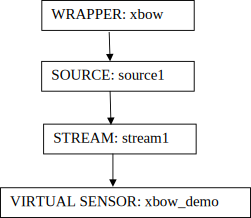
\includegraphics[width=0.4\columnwidth]{vs-dataflow}
  \caption{}
  \label{fig:tutorial-vs}
\end{figure}

\subsection{The multiFormatSample Virtual Sensor.}

We will use the MultiFormat wrapper
(src.gsn.wrappers.MultiFormatWrapper.java) since it is the simplest
wrapper to study (and modify) and the wrapper
\textquotedblleft{}simulates\textquotedblright{} a sensor which
provides temperature, light, and packet type sensor readings every
second but does not actually rely on an external data source for its
operation.

\subsection{Virtual Sensor Description File }

A \textbf{Virtual Sensor Description file} (\textit{VSD}) is an XML
file that contains the selection and the parameterization of the
\textit{VSP} and wrapper that compose a \textit{VS}.  This file also
contains the SQL statements that connect them together.

The multiFormatSample Virtual Sensor is defined by the following
virtual-sensor XML file:

\begin{xmlcode}[caption={multiFormatSample.xml}, label=listing:mfs-vs]
<virtual-sensor name="MultiFormatTemperatureHandler" priority="10">
	<processing-class>
		<class-name>gsn.vsensor.LightVirtualSensor</class-name>
		<init-params />
		<output-structure>
			<field name="light" type="double"/>
			<field name="temperature" type="double"/>
			<field name="packet_type" type="int/>
		</output-structure>
	</processing-class>
	<description>Simulates sensor readings every second.</description>
	<life-cycle pool-size="10" />
	<addressing>
		<predicate key="geographical">Sensor 114 @ EPFL</predicate>
		<predicate key="LATITUDE">46.520000</predicate>
		<predicate key="LONGITUDE">6.565000</predicate>			
	</addressing>
	<storage history-size="10"/>
	<streams>
		<stream name="input1">
			<source alias="source1" sampling-rate="1" storage-size="1">
				<address wrapper="multiformat">
					<predicate key="HOST">localhost</predicate>
					<predicate key="PORT">22001</predicate>
				</address>
				<query>SELECT light, temperature, timed FROM wrapper</query>
			</source>
 			<query>source1.light AS light_sensorFROM source1</query>
		</stream>
	</streams>
</virtual-sensor>
\end{xmlcode}


Listing  multiFormatSample.xml

\subsection{Wrapper}

A GSN Wrapper (Wrapper) is a piece of Java code that does the data
acquisition for a specific type of device..

The wrapper from which the data will be selected is defined in the
address element of the source, for example in multiFormatWrapper:

\begin{xmlcode}
				<address wrapper="multiformat">
					<predicate key="HOST">localhost</predicate>
					<predicate key="PORT">22001</predicate>
				</address>
\end{xmlcode}


The predicates included in the address element are parameters that are
particular to the wrapper used.  As the multiFormat wrapper generates
its own data the address predicates are not really required but are
included for illustration only.

In a wrapper that connects to an external data source, the predicates
contain parameters necessary to identify the instance of the wrapper to
be used.  In this case, if the wrapper connected to a real data sourse,
the parameters would define a network host address and port to connect
to the sensor.

The wrapper creates a table from the DataField[] structure:

\begin{xmlcode}[caption={DataField declaration in multiFormatWrapper.java}, label=listing:xml:data-field]
private DataField[] collection = new DataField[] { 
	new DataField("packet_type", "int", "packet type"), 
	new DataField("temperature", "double", "Presents the temperature sensor."),
	new DataField("light", "double", "Presents the light sensor.") };
\end{xmlcode}

When GSN is started, wrappers tables are given randomly generated
names, for example, the table for the MultiFormatWrapper in this
instance is given the name \_501577155. If we query that table (see),
we notice the following fields: timed, PACKET\_TYPE, TEMPERATURE,
LIGHT, and a primary key field PK. Some of the data fields are
automatically converted to upper case by GSN for clarity. These fields
correspond to the ones defined in the DataField[]array in the wrapper
code:

The timed field is automatically generated by GSN to indicate the
timestamp of the tuple. The timestamp is expressed in unix epoch time.

\begin{table*}[!htp]
	\centering
	{\normalfont\footnotesize
	\begin{tabulary}{\textwidth}{|C|C|C|C|J|}%
	\hline
		\multicolumn{5}{|c|}{\textbf{multiFormat Wrapper data table}} \\
	\hline
	\hline
		\textbf{PK} &
		\textbf{timed} &
		\textbf{PACKET\_TYPE } &
		\textbf{TEMPERATURE} &
		\textbf{LIGHT} \\
	\hline
	  386 & 1225841381231 & 1 &	NULL & 779 \\
	\hline
	  387 & 1225841382591 & 1 & NULL & 329.2 \\
	\hline
	\end{tabulary}
	}
	\caption{multiFormat Wrapper data table}
	\label{table:wrapper-table}
\end{table*}

Once the wrapper code is initialized and the wrapper table created
then when a virtual-sensor is loaded,  a view or a set of views is
created to represent the data source

\subsection{Source}

The source element of the VSD includes the wrapper declaration and an
SQL query to select the required data:

\begin{xmlcode} 	
<source alias="source1" sampling-rate="1" storage-size="1">
		<address wrapper="multiformat">
			<predicate key="HOST">localhost</predicate>
			<predicate key="PORT">22001</predicate>
		</address>
		<query>SELECT light, temperature, timed FROM wrapper</query>
	</source>
\end{xmlcode}

The attributes of the source include:

\textit{alias}\hspace{15pt}an identifier for this source

\textit{storage-size}\hspace{15pt}the window size - the number of data
items stored in the temporary table which sets the number of record
used to calculate aggregate functions such as AVG, MIN, MAX or SUM.  In
the example, no aggregate is used so the value is set at 1.  (In the
sample, two rows are present because the sample was viewed after a new
record was recieved but before the previous one was dropped.

\textit{slide}\hspace{15pt}the amount by which the sliding window
moves when generating aggregate queries.  For example, a slide value of
10 would generate a query on the arrival of each tenth record.  (slide
is not relevant to queries not using aggregate funcions such as the
present example.)

\textit{sampling-rate}\hspace{15pt}provides for load shedding when the
source generates data at a higher rate than required.  Has a value
between 0 and 1.  A value of 1 means no data is dropped, while a value
of 0.2 means only 20\% of data items will be processed and the
remainder (80\%) will be silently dropped.

The data view for source1 is named \_695753603and contains the
following data fields: light, temperature, packet type and timed (see
).

\begin{table*}[!htp]
	\centering
	{\normalfont\footnotesize
	\begin{tabulary}{\textwidth}{|C|C|C|J|}%
	\hline
		\multicolumn{4}{|c|}{\textbf{SELECT * FROM \_695753603;}} \\
	\hline
	\hline
		\textbf{light} &
		\textbf{temperature} &
		\textbf{packet\_type } &
		\textbf{timed} \\
	\hline
	  329.2 & NULL & 1 & 1225841382591\\
	\hline
	\end{tabulary}
	}
	\caption{Source data view}
	\label{table:source-view}
\end{table*}


Since views are virtual tables created by stored queries. This view
corresponds to the \textquotedblleft{}source\textquotedblright{} query
defined in the virtual-sensor XML file (). In this way, if several data
sources are declared, GSN can use views to
\textquotedblleft{}merge\textquotedblright{} data from wrapper tables,
in other words, views act as temporary tables to hold data used by
virtual-sensors.

\subsection{Stream}

A stream tells GSN what data to send to the result table created for
the virtual sensor.  The stream declaration defines the source views
from which data will be selected and the SQL query to select data to be
added to the table:

\begin{xmlcode}
<stream name="input1">
	<source alias="source1" sampling-rate="1" storage-size="1">
		<address wrapper="multiformat">
			<predicate key="HOST">localhost</predicate>
			<predicate key="PORT">22001</predicate>
		</address>
		<query>SELECT light, temperature, timed FROM wrapper</query>
	</source>
	<query>source1.light AS light_sensorFROM source1</query>
</stream>
\end{xmlcode}

The attributes of a stream include:

\textit{name}\hspace{15pt}a mandatory identifier for the stream.

\textit{rate}\hspace{15pt}The rate parameter is a performance tuning
parameter. It defines the minimum interval in milliseconds between two
calls to this virtual sensor. If there is data available for the
virtual sensor in less than this value, then the data is silently
dropped (Book of GSN p. 25).

\textit{count}\hspace{15pt}Count puts a limit on the life cycle of the
stream query in terms of number of outputs.

For instance, if the count is 100 it implies that the stream source
should become disabled after producing 100 values (stream elements).
This property is used rarely and it is planned to be 
removed from the next release. 

The stream query selects data from one or more sources and can perform
joins to combine data from multiple sources.  The result set of the
query is inserted into a table bearing the name of the virtual sensor
which becomes the output of the sensor.  The `timed' field can be
selected from one of the sources or failing that the time at the GSN
container host will be used.

\begin{table*}[!htp]
	\centering
	{\normalfont\footnotesize
	\begin{tabulary}{\textwidth}{|C|C|C|C|C|}%
	\hline
	\multicolumn{5}{|c|}{\textbf{SELECT * FROM multiformattemperaturehandler;}} \\
	\hline
	\textbf{PK} &
	\textbf{timed} &
	\textbf{LIGHT} &
	\textbf{TEMPERATURE} &
	\textbf{PACKET\_TYPE} \\
	\hline
  74552 &	1225841363432 &	 637.9 	&        NULL &	           1 \\ \hline
  74553 &	1225841364792 &	 507.3 	&        60.2 &	           2 \\ \hline
  74554 &	 1225841368402 &	  NULL &	     17.3 &	           2 \\ \hline
  74555 &	 1225841369042 &	 691.9 &       NULL &	           1 \\ \hline
  74556 &	 1225841372136 &	 380.3 &	     NULL &	           1 \\ \hline
  74557 &	 1225841375230 &	 834.5 &	     NULL &	           1 \\ \hline
  74558 &	 1225841376059 &	  NULL &	     60.1 &	           2 \\ \hline
  74559 &	 1225841378168 &	  NULL &	     75.7 &	           2 \\ \hline
  74560 &	 1225841381231 &	   779 &	     NULL &	           1 \\ \hline
  74561 &	 1225841382591 &	 329.2 &	     NULL &	           1 \\ \hline
	\end{tabulary}
	}
	\caption{multiFormat VS Output Table}
	\label{table:vs-out}
\end{table*}



\subsection{Virtual Sensor}

The root element of the VSD is labelled
\begin{math}<\end{math}virtual-sensor\begin{math}>\end{math} and
contains attributes that define the whole VS

\textit{name}\hspace{15pt}is a mandatory and arbitrary identifier for
the VS which can be used by another virtual sensor to idntify this
virtual sensor as a source using the remote or local virtual sensor
class.

\textit{priority}\hspace{15pt}is optional and must be between 0 which
is the highest priority and 20 is the lowest. The default priority is
10.

\subsubsection{Virtual Sensor Processing Class}

A \textbf{Virtual Sensor Processing class} (\textit{vsp}) is a piece
of Java code that process and stores the data upon reception from the
wrapper.

\begin{xmlcode}
	<processing-class>
		<class-name>gsn.vsensor.LightVirtualSensor</class-name>
		<init-params />
		<output-structure>
			<field name="light" type="double"/>
			<field name="temperature" type="double"/>
			<field name="packet_type" type="int/>
		</output-structure>
	</processing-class>
\end{xmlcode}
The key elements in this section are:

\textit{class-name}\hspace{15pt}specifies the name of a java class
that implements the virtual sensor processing class (VSP).
(gsn.vsensor.BridgeVirtualSensor is used in the example).  The GSN
distribution includes several VSP's and a framework in which others can
can be developed.

\textit{unique-timestamps}\hspace{15pt}allows the virtual sensor to
override the default which is to make the index to the timestamp
UNIQUE.  This would allow duplicated timestamps to be added to the
table.

\textit{init-params}\hspace{15pt}allows for the provision of
parameters to the virtual sensor class.  Parameters are specific to
individual sensor classes.

\textit{output-specification-rate} acts in a similar manner to the
rate attribute of a stream but presumably controls the the whole VS
rather than an individual stream.  In a VS with only one stream both
seem to have the same effect which is to pevent the generation of
another data row until the specified time (in milliseconds) has
elapsed.

\textit{output-structure}\hspace{15pt}provides the structure of a row
in the output data.  The name and type attributes of each field element
must match those of a data item selected in the stream query.  The text
contents of each field element can contain an optional description of
the field.

\subsubsection{Other Elements of a VSD}

Other elements of the \textit{VSD} include:

\textit{description }can contain a textual description of the sensor.

\textit{life-cycle pool-size }is a performance parameter.  It is
usually safe to keep the default value.  It defines the maximum number
of instances of this virtual sensor (with this configuration). This can
happen when the processing method of the virtual sensor takes a long
time to complete, and / or when data arrives at high speed. If all
instances are busy, then the data will be dropped.

The \textit{addressing} element contains predicates which can be used
to specify the location and other characteristics of the virtual
sensor.  The predefined keys
\textquotedblleft{}LATITUDE\textquotedblright{} and
\textquotedblleft{}LONGITUDE\textquotedblright{} can be used to locate
the sensor on the map pages of the web interface.

\textit{storage history-size} sets the number of records to be
retained in the virtual sensor table.  It does not impact the logical
processing of data streams.

\subsection{Summary}

The multiFormatSample VS is a very simple example which simply selects
data fields in the stream from a single wrapper.  The examples were
generated using release 890 of GSN and MySQL as the underlying
database.

The real power of GSN lays in its ability to use more complex SQL
queries with multiple data streams, sources and wrappers but that can
only be approached with any confidence once the basics are understood.


\newpage

	\chapter{GSN in Nutshell}%: Stream Processing Infrastructure for Large-scale Interconnected Streaming World


\section*{Abstract}
  With the price of wireless sensor technologies diminishing rapidly we can
  expect large numbers of autonomous sensor networks being deployed in the near
  future. These sensor networks will typically not remain isolated but the need
  of interconnecting them on the network level to enable integrated data
  processing will arise, thus realizing the vision of a global ``Sensor
  Internet.'' This requires a flexible middleware layer which abstracts from
  the underlying, heterogeneous sensor network technologies and supports fast
  and simple deployment and addition of new platforms, facilitates efficient
  distributed query processing and combination of sensor data, provides support
  for sensor mobility, and enables the dynamic adaption of the system
  configuration during runtime with minimal (zero-programming) effort. This
  paper describes the Global Sensor Networks (GSN) middleware which addresses
  these goals. We present GSN's conceptual model, abstractions, and
  architecture, and demonstrate the efficiency of the implementation through
  experiments with typical high-load application profiles. The GSN
  implementation is available from \url{http://gsn.sourceforge.net/}.
\newpage
\section*{Related Publications:}
Different parts of the work presented in this chapter is published in the form of articles in international conferences and workshops.
Parts of this chapter is also published in the form of internal technical reports.
\begin{itemize}
\item \emph{Infrastructure for data processing in large-scale interconnected sensor networks}, Karl Aberer , Manfred Hauswirth , Ali Salehi. Mobile Data Management (MDM), Germany, 2007.
\item \emph{GSN, Quick and Simple Sensor Network Deployment}, Ali Salehi, Karl Aberer. European conference on Wireless Sensor Networks (EWSN), Netherlands, 2007.
\item \emph{Zero-programming Sensor Network Deployment}, Karl Aberer , Manfred Hauswirth , Ali Salehi. Next Generation Service Platforms for Future Mobile Systems (SPMS), Japan, 2007.
\item \emph{A middleware for fast and flexible sensor network deployment}, Karl Aberer , Manfred Hauswirth , Ali Salehi. Very Large Data Bases (VLDB) Seoul, Korea, 2006.
\item \emph{Middleware support for the "Internet of Things"}, Karl Aberer , Manfred Hauswirth , Ali Salehi. 5. GI/ITG KuVS Fachgesprch "Drahtlose Sensornetze", Universitt Stuttgart, 2006.
\item \emph{The Global Sensor Networks middleware for efficient and flexible deployment and interconnection of sensor networks}, Karl Aberer , Manfred Hauswirth , Ali Salehi.
Technical Report, LSIR-2006-006.
\item \emph{Global Sensor Networks}, Karl Aberer , Manfred Hauswirth , Ali Salehi. Technical Report, LSIR-2006-001.
\end{itemize}
\newpage
\section{Introduction}
\label{sec:introduction}

Until now, research in the sensor network domain has mainly focused on
routing, data aggregation, and energy conservation inside a single
sensor network while the integration of multiple sensor networks has
only been studied to a limited extent. However, as the price of
wireless sensors diminishes rapidly we can soon expect large numbers
of autonomous sensor networks being deployed. These sensor networks
will be managed by different organizations but the interconnection of
their infrastructures along with data integration and distributed
query processing will soon become an issue to fully exploit the
potential of this ``Sensor Internet.'' This requires platforms which
enable the dynamic integration and management of sensor networks and
the produced data streams.

The Global Sensor Networks (GSN) platform aims at providing a flexible
middleware to accomplish these goals.  GSN assumes the simple model
shown in Figure~\ref{fig:setup}: A sensor network internally may use
arbitrary multi-hop, ad-hoc routing algorithms to deliver sensor
readings to one or more sink node(s). A sink node is a node which is
connected to a more powerful base computer which in turn runs the GSN
middleware and may participate in a (large-scale) network of base
computers, each running GSN and servicing one or more sensor networks.

\begin{figure}
  \centering
  \includegraphics[width=0.5\columnwidth]{ch-gsn-figures/model}
  \caption{GSN model}
  \label{fig:setup}
\end{figure}

We do not make any assumptions on the internals of a sensor network
other than that the sink node is connected to the base computer via a
software wrapper conforming to the GSN API. On top of this physical
access layer GSN provides so-called \textit{virtual sensors} which
abstract from implementation details of access to sensor data and
define the data stream processing to be performed. Local and remote
virtual sensors, their data streams and the associated query
processing can be combined in arbitrary ways and thus enable the user
to build a data-oriented ``Sensor Internet'' consisting of sensor
networks connected via GSN.

In the following we start with a detailed description of the virtual
sensor abstraction in Section~\ref{sec:virt-sens-spec}, discuss GSN's
data stream processing and time model in
Section~\ref{sec:data-stre-proc}, and present GSN's system architecture
along with a discussion of essential implementation details
in Section~\ref{sec:system-architecture}. We
evaluate the performance of GSN in Section~\ref{sec:evaluation} and
discuss related work in Section~\ref{sec:relatedwork} before
concluding.

\section{Virtual sensors}
\label{sec:virt-sens-spec}

The key abstraction in GSN is the \textit{virtual sensor}. Virtual
sensors abstract from implementation details of access to sensor data
and correspond either to a data stream received directly from sensors
or to a data stream derived from other virtual sensors. A virtual
sensor can be any kind of data producer, for example, a real sensor, a
wireless camera, a desktop computer, or any combination of virtual sensors.
A virtual sensor may have any number of input data
streams and produces exactly one output data stream (with predefined format) based on the input
data streams and arbitrary local processing. The specification of a
virtual sensor provides all necessary information required for
deploying and using it, including (1) metadata used for identification
and discovery, (2) the details of the data streams which the virtual
sensor consumes and produces (3) an SQL-based specification of the
stream processing (filtering and integration) performed in a virtual sensor, (4)
the processing class which preforms the more advanced and complex data processing (if needed) on the output
stream before releasing it and (5) functional properties related to persistency, error handling, life-cycle,
management, and physical deployment.

To support rapid deployment, the virtual sensors are provided
in human readable declarative forms (XML). Figure~\ref{fig:ComplexVS} shows an
example which defines a virtual sensor that reads two temperature sensors and
in case both of them have the same reading above a certain threshold in the
last minute, the virtual sensor returns the latest picture from the webcam in
the same room together with the measured temperature.


\begin{figure}%[htb]
  \centering
  \lstset{numbers=left, numberstyle=\footnotesize}
\begin{lstlisting}
<virtual-sensor name="room-monitor" priority="10" 
         protected="false" >
  <processing-class>
     <class-name>gsn.vsensor.BridgeVirtualSensor</class-name>
     <init-params/>
     <output-structure>
        <field name="image" type="binary:jpeg" />
        <field name="temp"  type="int" />
     </output-structure>
  </processing-class>
  <life-cycle pool-size="10" />
  <addressing>
      <predicate key="geographical">BC143</predicate>
      <predicate key="usage">room monitoring</predicate>
      <predicate key="latitude">46.5214</predicate>
      <predicate key="longitude">6.5676</predicate>
  </addressing>
  <storage history-size="10h" />
  <streams>
      <stream name="cam">
         <source name="cam"  storage-size="1" >
            <address wrapper="remote">
               <predicate key="geographical">BC143</predicate>
               <predicate key="type">Camera</predicate>
            </address>
            <query>select * from WRAPPER</query>
         </source>
         <source name="temperature1" storage-size="1m" >
            <address wrapper="remote">
               <predicate key="type">temperature</predicate>
               <predicate key="geographical">BC143-N</predicate>
            </address>
            <query>select AVG(temp1) as T1 from WRAPPER</query>
         </source>
         <source name="temperature2"  storage-size="1m" >
            <address wrapper="remote">
               <predicate key="type">temperature</predicate>
               <predicate key="geographical">BC143-S</predicate>
            </address>
            <query>select AVG(temp2) as T2 from WRAPPER</query>
         </source>
         <query>
            select cam.picture as image, temperature.T1 as temp
            from   cam, temperature1
            where  temperature1.T1 > 30 AND
                   temperature1.T1 = temperature2.T2
         </query>
      </stream>
   </streams>
</virtual-sensor>
\end{lstlisting}
  \caption{A virtual sensor definition}
  \label{fig:ComplexVS}
\end{figure}

A virtual sensor has a unique name (the \verb|name| attribute in line 1) and
can be equipped with a set of key-value pairs representing the logical addressing of the
virtual sensor (lines 12--17), i.e., associated with metadata. The addressing information can be registered and
discovered in GSN and other virtual sensors can use either the unique name or
logical addressing based on the metadata to refer to a virtual sensor. 
We have defined certain addressing keys which are specifically used by the GSN's web interface. In GSN if a given
virtual sensor has the addressing values for the both \texttt{latitude} (line 15) and \texttt{longitude} (line 16) keys, the default GSN
web interface uses these geographical locations to show the sensor on the global map.

The example specification above defines a virtual sensor with three input streams
which are identified by their metadata\footnote{Note that the support for distributed directory/registry service had been removed
from GSN's source code thus as of \today, we only support physical addressing for identifying the data sources.},
i.e., by logical addressing. For example, the first temperature sensor is
addressed by specifying two requirements on its metadata, namely
that it is of type temperature sensor and at a certain physical certain
location. By using multiple input streams Figure \ref{fig:ComplexVS} also
demonstrates GSN's ability to access multiple stream producers simultaneously.
For the moment, we assume that the input streams (two temperature sensors and a
webcam) have already been defined in other virtual sensor definitions (how this
is done, will be described below).

In GSN data streams are temporal sequences of timestamped tuples (also known as \texttt{Stream Elements}).
This is in line with the model used in most stream processing systems. The structure of
the output data stream a virtual sensor produces is encoded in XML as shown in lines 6 -- 9 (the \texttt{output-structure} part).
The structure of the input streams is learned from the respective specifications of their virtual sensor definitions. 

In GSN data stream processing is separated into three stages:
\begin{itemize}
\item processing applied to sources (lines 26, 33, and 40).
\item processing for combining data from the different input streams and producing the temporary output stream (lines 43-46).
\item producing the final output stream by passing the temporary output stream from a processing class (a processing logic represented in some programming languages). This part is presented by lines 3 -- 10. Note that as the final output is produced by the processing class, the actual output structure of the virtual sensor should strictly
conform the output format of the processing class \footnote{As of \today, the order and the types should be exactly match.}.
\end{itemize}

To specify the processing of the sources we use SQL queries which refer to the actual data source
by the reserved keyword \verb|WRAPPER| (the data sources are logically represented as relational tables all of which called \verb|wrapper|).
The attribute \verb|wrapper="remote"| indicates that the data stream is obtained through the
network from another virtual sensor which can be located in any other GSN instance accessible through the network.


In the case of a directly connected local sensor, the \verb|wrapper| attribute would reference the required wrapper\footnote{As of \today, all the wrappers has to written in Java language. The actual code for accessing the sensor can be written in any language as long as there is a possibility of communicating the data to the hardware
through Java (e.g., interfacing Java to existing C code or the serial ports).}.
For example, \verb|wrapper="tinyos"| would denote a TinyOS-based sensor whose data
stream is accessed via GSN's TinyOS wrapper \footnote{In GSN, we have multiple TinyOS wrappers each corresponding to different
versions and packet formats. Those details are out of the score of this chapter.}.
GSN already includes wrappers for all major TinyOS platforms (Mica2, Mica2Dot, etc.), for wired and wireless
(HTTP-based) cameras (e.g., AXIS 206W), several RFID readers (Texas
Instruments, Alien Technology), Bluetooth devices, Shockfish, WiseNodes, epuck
robots, etc. The implementation effort for wrappers is rather low, for example,
the RFID reader wrapper has 50 lines of code (LOC), the TinyOS wrapper has 120
LOC, and the generic serial wrapper has 180 LOC.

In the given example the output stream joins the data received from two
temperature sensors and returns a camera image if certain conditions on the
temperature are satisfied (lines 43--46). To enable the SQL statement in lines
43--46 to produce the output stream, it needs to be able to reference the
required sources which is accomplished by the \verb|name| attribute
(lines 21, 28, and 35) that defines a symbolic name for each stream source.

The definition of the structure of the output stream directly relates to the data
stream processing that is performed by the virtual sensor's processing class and needs to be
consistent with it. GSN provides multiple processing classes each of which are designed
to perform different tasks (e.g., charts, network plots, filtering, ...). In our example we are using
\texttt{gsn.vsensor.BridgeVirtualSensor} as our processing class. The \texttt{gsn.vsensor.BridgeVirtualSensor}
class is special in the sense that unlike most of the other GSN's processing classes, this class does not
perform any further processing on its input stream thus it does not alter the data nor the structure of its input.

Since the structure of the virtual sensor output is not altered through using the \texttt{gsn.vsensor.BridgeVirtualSensor} processing class hence the final
structure of the virtual sensor's output is determined through the SQL statement at line 43, we need to make sure that,
the data fields in the \verb|select| clause matches the definition of the output structure in lines 6--9 (the order is important).
It is recommended to use \texttt{gsn.vsensor.BridgeVirtualSensor} as long as the processing preformed in the virtual
sensor through the SQL queries are sufficient enough and no further processing is required before publishing the sensor 
data to the outside.

In the design of GSN specifications we decided to separate the temporal aspects
from the relational data processing using SQL. The temporal processing is
controlled by various attributes provided in the input and output stream
specifications, e.g., the attribute \verb|storage-size| (lines 21, 28, and 35)
defines the window size used for producing the input stream's data elements.
Due to its specific importance the temporal processing will be discussed in
detail in Section~\ref{sec:data-stre-proc}.

In addition to the specification of the data-related properties a virtual
sensor also includes high-level specifications of functional properties: The
\verb|priority| attribute (line 1) controls the processing priority of a
virtual sensor, the \verb|<life-cycle>| element (line 11) enables the control
and management of resources provided to a virtual sensor such as the maximum
number of threads/queues available for processing, the \verb|<storage>| element
(line 18) allows the user to control how output stream data is persistently
stored.

For example, in Figure~\ref{fig:ComplexVS} the \verb|priority| attribute in
line 1 assigns a priority of 10 to this virtual sensor (1 is the lowest
priority and 20 the highest, default is 10), the \verb|<life-cycle>| element in
line 11 specifies a maximum number of 10 threads, which means that if the pool
size is reached, data will be dropped (if no pool size is specified, it will be
controlled by GSN depending on the current load), the \verb|<storage>| element
in line 18 defines that the output stream's data elements of the last 10 hours
(\verb|history-size| attribute) are stored to enable off-line processing.
The \verb|storage-size| attribute in line 21 defines the window size of 1 stream element. That's the most recent
image taken by the webcam irrespective of the time it was
taken.

In GSN, we can specify the set of values either by time or count. In the count based representation
one only presents the values through integers. For instance \verb|slide='2'| or \verb|history-size='100'|. The count based representation is consists of
an integer directly postfixed (without any space characters) with one of the time measurement units. As of \today, we have \texttt{d},\texttt{h},\texttt{m},\texttt{s} time measurement units which are corresponding to days, hours, minutes and seconds. As a time based example, we might have \verb|storage-size='1m'|.

The \verb|storage-size| attributes in lines 28 and 35 define a window of one minute for the amount of sensor readings subsequent queries
will be run on, i.e., the \verb|AVG| operations in lines 33 and 40 are executed
on the sensor readings received in the last minute which of course depends on
the rate at which the underlying temperature virtual sensor produces its
readings. Note that when the \verb|storage-size| is anything other than \emph{1}, the
virtual sensor author should be aware of the possibility of duplicated stream elements (discussed in more
detail in section \ref{sec:data-stre-proc}).

The query producing the output stream (lines 43--46) also demonstrates another
interesting capability of GSN as it also mediates among three different flavors
of queries: The virtual sensor itself uses continuous queries on the
temperature data, a ``normal'' database query on the camera data and
produces a result only if certain conditions are satisfied, i.e., a
notification analogous to pub/sub or active rules.

Virtual sensors are a powerful abstraction mechanism which enables the user to
declaratively specify sensors and combinations of arbitrary complexity. Virtual
sensors can be defined and deployed to a running GSN instance at any time
without having to stop the system. Also dynamic unloading is supported but
should be used carefully as unloading a virtual sensor may have undesired
(cascading) effects. 

\section{Data stream processing and time model}
\label{sec:data-stre-proc}

Data stream processing has received substantial attention in the
recent years in other application domains, such as network monitoring
or telecommunications. As a result, a rich set of query languages and
query processing approaches for data streams exist on which we can
build. A central building block in data stream processing is the time
model as it defines the temporal semantics of data and thus determines
the design and implementation of a system. Currently, most stream
processing systems use a global reference time as the basis for their
temporal semantics because they were designed for centralized
architectures in the first place. As GSN is targeted at enabling a
distributed ``Sensor Internet,'' imposing a specific temporal semantics
seems inadequate and maintaining it might come at unacceptable cost.
GSN provides the essential building blocks for dealing with time, but
leaves temporal semantics largely to applications allowing them to
express and satisfy their specific, largely varying requirements. In
our opinion, this pragmatic approach is viable as it reflects the
requirements and capabilities of sensor network processing.

In GSN a data stream is a set of timestamped tuples also known as Stream Elements.
The order of the data stream is derived from the ordering of the timestamps and GSN
provides basic support for managing and manipulating the timestamps.
The following essential services are provided:

\begin{enumerate}
\item a local clock at each GSN Server
\item implicit management of a timestamp attribute (reserved field called \texttt{TIMED})\footnote{All timestamps in GSN are represented in milliseconds using 64-bit integers.}\footnote{As the timestamp (e.g., the \texttt{TIMED} field) is always present, it is not required to specify the \texttt{TIMED} field in the  \texttt{output-structure} section of the virtual sensors. In fact, specifying the \texttt{TIMED} field in the output structure causes error therefore GSN refuses to load the virtual sensor.}
\item automatic timestamping of tuples upon arrival at the GSN in case the tuples (stream elements) don't have
any timestamp (no \texttt{TIMED} field available)
\item a windowing mechanism which allows the user to define count- or
  time-based windows on data streams.
\item a sliding mechanism which allows the user to define count- or  time-based sliding behaviors on data streams.
\end{enumerate}

In this way it is always possible to trace the temporal history of
data stream elements throughout the processing history.  Multiple time
attributes can be associated with data streams (as long as only one of them called \texttt{TIMED})
and can be manipulated through SQL queries. Thus sensor networks can be used as observation
tools for the physical world, in which network and processing delays
are inherent properties of the observation process which cannot be
made transparent by abstraction.  Let us illustrate this by a simple
example: Assume a bank is being robbed and images of the crime scene
taken by the security cameras are transmitted to the police. For the
insurance company the time at which the images are taken in the bank
will be relevant when processing a claim, whereas for the police
report the time the images arrived at the police station will be
relevant to justify the time of intervention. Depending on the context
the robbery is thus taking place at different times.

As tuples (sensor readings) are timestamped, queries can also deal
explicitly with time. For example, the query in lines 43--46 of
Figure~\ref{fig:ComplexVS} could be extended such that it explicitly
specifies the maximum time interval between the readings of the two
temperatures and the maximum age of the readings. This would
additionally require changes in the source definitions as the
sources then must provide this information (more detailed example below), and also the
averaging of the temperature readings (lines 33 and 40) would have to
be changed to be explicit in respect to the time dimension.

In order to concretely show the time management inside GSN, we would like to
simulate above scenario through two different virtual sensors (only the input stream parts presented).
Say there exist a virtual sensor called \emph{camera-vs} hosted on a GSN server which listens to port \texttt{80} on a machine with IP address of \texttt{1.2.3.4}.
The virtual sensor used by the police and the one used by the insurance are depicted in figures \ref{vs:police} and \ref{vs:insurance}.
The stream specified in figure \ref{vs:police} has a query in line 7 for retrieving both the picture and the time stamp from the remote virtual sensor therefore
the remote timestamp is used by GSN for the internal calculations. Now consider the stream specified in figure \ref{vs:insurance} which has a small change compared to the one in figure \ref{vs:police}, the latter is not selecting the timestamp field hence GSN automatically adds the local reception time to every tuple it receives from the remote source.

In order to further elaborate the time management issue, consider the stream source specified in figure \ref{vs:complex-time}. This example combines both
the local time and remote time in order to measure the latency associated with each tuple and uses the latency as a condition as the selection
criteria (e.g., only accepting the tuples which are not delayed by the network for more than 5 milliseconds).

\begin{figure}%[htb]
  \centering
  \lstset{numbers=left, numberstyle=\footnotesize}
\begin{lstlisting}
<stream name="cam">
   <source name="cam"  storage-size="1" >
      <address wrapper="remote">
         <predicate key="host">1.2.3.4</predicate>
         <predicate key="port">80</predicate>
         <predicate key="name">camera-vs</predicate>
      </address>
      <query>select PICTURE, TIMED from WRAPPER</query>
   </source>
	 <query>
      select PICTURE, TIMED from cam
   </query>
</stream>
\end{lstlisting}
  \caption{A stream using the remote timestamp.}
  \label{vs:police}
\end{figure}

\begin{figure}%[htb]
  \centering
  \lstset{numbers=left, numberstyle=\footnotesize}
\begin{lstlisting}
<stream name="cam">
   <source name="cam"  storage-size="1" >
      <address wrapper="remote">
         <predicate key="host">1.2.3.4</predicate>
         <predicate key="port">80</predicate>
         <predicate key="name">camera-vs</predicate>
      </address>
      <query>select PICTURE from WRAPPER</query>
   </source>
   <query>
      select PICTURE, TIMED from cam
   </query>
</stream>
\end{lstlisting}
 \caption{A stream using the local (arrival) timestamp.}
  \label{vs:insurance}
\end{figure}

\begin{figure}%[htb]
  \centering
  \lstset{numbers=left, numberstyle=\footnotesize}
\begin{lstlisting}
<stream name="cam">
   <source name="cam"  storage-size="1" >
      <address wrapper="remote">
         <predicate key="host">1.2.3.4</predicate>
         <predicate key="port">80</predicate>
         <predicate key="name">camera-vs</predicate>
      </address>
      <query>select PICTURE, TIMED as REMOTE_TIMED from WRAPPER</query>
   </source>
   <query>
      select PICTURE, REMOTE_TIMED AS TIMED from cam where 
      (cam.TIMED - cam.REMOTE_TIMED) < 5
   </query>
</stream>
\end{lstlisting}
   \caption{A stream using both local and remote timestamps.}
  \label{vs:complex-time}
\end{figure}

\begin{figure}
  \centering
  
\includegraphics[width=1\columnwidth]{ch-gsn-figures/sliding-window-visually}
  \caption{Illustration of the different sample sliding and window values.}
  \label{fig:sliding-window-visually}
\end{figure}

In order to deal with the streaming data, the standard way is to specify
a query with at least two extra properties associated with it,
window size and sliding value. The window size is used to limit
the actual data used for the processing (execution)  to a certain range
in time or number of values. The sliding value is introduced to
specify the execution condition for the query. The execution of the
query is triggered whenever the sliding condition is satisfied implying a possibly infinitely long periodic
execution of the query, therefore in stream processing systems, continuous queries are executed whenever the sliding occurs.

For instance, one can express the interest
of obtaining the average of a temperature sensor over the last $10$
minutes, and doing so periodically every $2$ minutes, by simply
providing the window size of $10$ minutes and sliding value of $2$
minutes to the stream processing engine. As indicated before, each
time the sliding condition is satisfied (e.g., $2$ minutes passed from
the previous execution) the actual action, computing the average over the last $10$
minutes, is performed. Note that in some research papers the
execution of the action is also called \emph{movement of the sliding
window}. 

The temporal processing in GSN is defined using the sliding and window values. Every data source in
GSN can have at most one \verb|slide|\footnote{Default value is 1, therefore this attribute can be omitted}
and \verb|storage-size|\footnote{No default value defined} attributes. Both values can be represented
in the form of count-based or time-based values (described earlier in this section).
Figure \ref{fig:sliding-window-visually} visually represents the query execution inside GSN with different sliding and window values.
We used a black dot in the figure to represent the triggering of execution. For instance, if both the window size and the sliding 
values are 3, and say we have received 5 stream elements in total, our continuous query have been executed only once (at the \emph{Time 3}) during its life time. 
One can extend above paradigm to create virtual sensors to support the integration of continuous and
historical data. For example, if the user wants to be notified when the temperature is 10 degrees above the average temperature in the
last 24 hours, he/she can simply define two sources, getting data from the same wrapper but with different window sizes, i.e., 1
(count) and 24h (time), and then simply write a query specifying the original condition with these sources.


The production of a new output stream element of a virtual sensor is always triggered
by the arrival of a data stream element from one of its input streams, thus processing is event-driven.
As described before, a stream can have multiple sources. 
Once the window of one of the sources of a stream slides, the 
following processing steps are performed:

\begin{enumerate}
%\item By default the new data stream element is timestamped using the local
%  clock of the virtual sensor provided that the stream element had no
%  timestamp.
\item Based on the timestamps for each stream the stream elements are
  selected according to the definition of the time window and the resulting
  sets of relations are unnested into flat relations.
\item The queries defined on the source are evaluated and stored into temporary
  relations.
\item The stream query for producing the input of the processing class is executed
  based on the temporary relations.
\item The resulted stream elements are forwarded to the processing class.
\item The output of the processing class is stored and simultaneously forwarded (notification) to
 all consumers of the virtual sensor.
\end{enumerate}

Figure~\ref{fig:ConceptualDataFlow} shows the logical data flow inside
a GSN node.

\begin{figure}%[htb]
  \centering
  \includegraphics[width=0.7\columnwidth]{ch-gsn-figures/conceptual-dataflow}
  \caption{Conceptual data flow in a GSN node}
  \label{fig:ConceptualDataFlow}
\end{figure}

Additionally, GSN provides a number of attributes in the virtual sensor file to control data rates.
The values used for controlling these rates are usually float numbers between 0 to 1.
The data rate controlling is useful whenever one wants to drop the stream elements with some random probability for load shedding. 
For instance, if one has a temperature source that keeps producing 
data with very high rate, one might want to sample the produced values 
thus making the processing lighter. For instance if one sets the 
sampling-rate to 0.75, any received stream element from the wrapper is going to be 
included in the window (the window and sliding values are explained above) with a probability of 75 out of 100.
Thus, on average 25 random stream elements will be dropped out of the last 100 elements.
In most of the cases one typically sets the rate control attributes to "1" to make sure nothing is dropped.

The rate control can be applied in the following three different levels (please refer to the virtual sensor quick reference for the syntactical
information about different portions of the virtual sensor file):
\begin{itemize}
\item At the source level by providing \texttt{sampling-rate} attribute (float value in [0 .. 1]).
\item At the stream level by providing \texttt{rate} attribute (integer value above zero).
\item At the virtual sensor output level by providing \texttt{output-specification} $\rightarrow$ \texttt{rate} attribute (integer value above zero).
\end{itemize}

As noted above, if the rate control is a positive integer, it defines the minimum allowed time difference between to successive stream elements.
For instance, if one is interested in receiving an average of a given sensor once an hour but the sensor underneath can produce arbitrary number of stream elements 
(e.g., due to uncontrollable packet losses in the internal network), he can express this behavior by setting the rate attribute of the virtual sensor output 
(\texttt{output-specification} $\rightarrow$ \texttt{rate}) to ``3600000'' (one hour is 3,600,000 milliseconds).

To specify the data stream processing a suitable language is needed. A number
of proposals exist already, so we compare the language approach of GSN to the
major proposals from the literature. In the Aurora project~\cite{Cherniack03}
(\url{http://www.cs.brown.edu/research/aurora/}) users can compose stream
relationships and construct queries in a graphical representation which is then
used as input for the query planner.  The Continuous Query Language (CQL)
suggested by the STREAM project~\cite{Arasu06}
(\url{http://www-db.stanford.edu/stream/}) extends standard SQL syntax with new
constructs for temporal semantics and defines a mapping between streams and
relations. Similarly, in Cougar~\cite{Yao03}
(\url{http://www.cs.cornell.edu/database/cougar/}) an extended version of SQL
is used, modeling temporal characteristics in the language itself. The
StreaQuel language suggested by the TelegraphCQ project~\cite{Chandrasekaran03}
(\url{http://telegraph.cs.berkeley.edu/}) follows a different path and tries to
isolate temporal semantics from the query language through external definitions
in a C-like syntax. For example, for specifying a sliding window for a query a
\textit{for}-loop is used. The actual query is then formulated in an SQL-like
syntax.

GSN's approach is related to TelegraphCQ's as it separates the
time-related constructs from the actual query. Temporal
specifications, e.g., the window size and rates, are specified in XML in the
virtual sensor specification, while data processing is specified in
SQL. Using this design, GSN can support SQL queries with the full range of
operations allowed by the standard SQL syntax, i.e., joins,
sub-queries, ordering, grouping, unions, intersections, etc.
The advantage of using SQL is that it is well-known and SQL query
optimization and planning techniques can be directly applied.

\section{System architecture}
\label{sec:system-architecture}

GSN uses a container-based architecture for hosting virtual sensors.
Similar to application servers, GSN provides an environment in which
sensor networks can easily and flexibly be specified and deployed by
hiding most of the system complexity in the GSN Server.  Using the
declarative specifications, virtual sensors can be deployed and
reconfigured in GSN Servers at runtime. Communication and
processing among different GSN Servers is performed in a
peer-to-peer style through standard Internet and Web Services protocols. By
viewing GSN Servers as cooperating peers in a decentralized system,
we tried avoid some of the intrinsic scalability problems of many
other systems which rely on a centralized or hierarchical
architecture. Targeting a ``Sensor Internet'' as the long-term goal we
also need to take into account that such a system will consist of
``Autonomous Sensor Systems'' with a large degree of freedom and only
limited possibilities of control, similarly as in the Internet.

Figure~\ref{fig:NodeArchitecture} shows the layered architecture of a
GSN Server.

\begin{figure}%[htb]
  \centering
  \includegraphics[width=0.45\columnwidth]{ch-gsn-figures/NodeArchitecture}
  \caption{GSN Server architecture}
  \label{fig:NodeArchitecture}
\end{figure}

Each GSN server hosts a number of virtual sensors it is responsible
for. The virtual sensor manager (VSM) is responsible for providing
access to the virtual sensors, managing the delivery of sensor data,
and providing the necessary administrative infrastructure. The VSM has
two subcomponents: The life-cycle manager (LCM) provides and manages
the resources provided to a virtual sensor and manages the
interactions with a virtual sensor (sensor readings, etc.). The input
stream manager (ISM) is responsible for managing the streams,
allocating resources to them, and enabling resource sharing among them
while its stream quality manager subcomponent (SQM) handles sensor
disconnections, missing values, unexpected delays, etc., thus ensuring
the QoS of streams. All data from/to the VSM passes through the
storage layer which is in charge of providing and managing persistent
storage for data streams. Query processing in turn relies on all of
the above layers and is done by the query manager (QM) which includes
the query processor being in charge of SQL parsing, query planning,
and execution of queries (using an adaptive query execution plan). The
query repository manages all registered queries (subscriptions) and
defines and maintains the set of currently active queries for the
query processor.  The notification manager deals with the delivery of
events and query results to registered, local or remote virtual sensors. The
notification manager has an extensible architecture which allows the
user to largely customize its functionality, for example, having
results mailed or being notified via SMS.

The top three layers of the architecture deal with access to the GSN
server. The interface layer provides access functions for other GSN
servers and via the Web (through a browser or via web services).
These functionalities are protected and shielded by the access control
layer providing access only to entitled parties and the data integrity
layer which provides data integrity and confidentiality through
electronic signatures and encryption. Data access and data integrity
can be defined at different levels, for example, for the whole GSN
server or at a virtual sensor level.

In connection with RFID tags this ``plug-and-play'' feature of GSN
provides new and interesting types of mobility which we will
investigate in future work. For example, an RFID tag may store queries
which are executed as soon as the tag is detected by a reader, thus
transforming RFID tags from simple means for identification and
description into a GSN server for physically mobile queries which opens
up new and interesting possibilities for mobile information systems.

%\section{Self Identifying Devices}
%An interesting feature of GSN's architecture is the support for sensor
%mobility based on automatic detection of sensors and zero-programing
%deployment: A large number of sensors already support the IEEE 1451
%standard which describes a sensor's properties and measurement
%characteristics such as type of measurement, scaling, and calibration
%information in a so-called Transducer Electronic Data Sheet (TEDS)
%which is stored inside the sensor. When a new sensor node is detected
%by GSN, for example, by moving into the transmission range of a sink
%node, GSN requests its TEDS and uses the contained information for the
%dynamic generation of a virtual sensor description by using a virtual
%sensor description template and deriving the sensor-specific fields
%of the template from the data extracted from the TEDS. At the moment
%TEDS provides only that information about a sensor which enables
%interaction with it.  Thus for some parts of the generated virtual
%sensor description, e.g., security requirements, storage and resource
%management, etc., we use default values. Then GSN dynamically
%instantiates the new virtual sensor based on this synthesized
%description and all local and remote processing dependent on the new
%sensor is executed. This is done on-the-fly while GSN is running. The
%inverse process is performed if a sensor is no longer associated with
%a GSN node, e.g., it has moved away.

\section{Implementation}
\label{sec:implementation}

The GSN implementation consists of the GSN-CORE, implemented in Java, and the
platform-specific GSN-WRAPPERS, implemented in Java, C, and Ruby, depending on
the available toolkits for accessing specific types of sensors or sensor
networks. The implementation currently has approximately 80,000 lines of code
and is available from SourceForge (\url{http://gsn.sourceforge.net/}). GSN
is implemented to be highly modular in order to be deployable on various
hardware platforms from workstations to small programmable PDAs, i.e.,
depending on the specific platforms only a subset of modules may be used. GSN
also includes visualization systems for plotting data and visualizing the
network structure. In the following sections we are going to discuss some of
the key aspects of the GSN implementation

\subsection{Adding new sensor platforms}
\label{sec:adding-new-sensor}

For deploying a virtual sensor the user only has to specify an XML document as described in Section \ref{sec:virt-sens-spec}, if GSN already
includes software support for the concerned hardware/software. Adding a new
type of sensor or sensor network can be done by supplying the name of the wrapper (specified in \texttt{/conf/wrappers.properties})
conforming to the GSN API. At the moment GSN provides the following wrappers:

\begin{description}
\item[HTTP generic wrapper] is used to pull data from devices via HTTP GET
  or POST requests, for example, the AXIS206W wireless camera.

\item[TinyOS wrapper] enables interaction with TinyOS compatible
motes (version 1.x and 2.x). This wrapper uses the serial forwarder which is
the standard access tool for TinyOS provided in the TinyOS package.

\item[USB camera wrapper] is used for dealing with cameras connected via USB 
  to the local machine. As USB cameras are very cheap, they are quite
  popular as sensing devices. The wrapper supports cameras
  with OV518 and OV511 chips (see \url{http://alpha.dyndns.org/ov511/}).
  
\item[TI-RFID wrapper] enables access to Texas Instruments Series 6000 S6700
  multi-protocol RFID readers.

\item[Generic UDP wrapper] can be used for any device using the UDP protocol to
  send data.
  
\item[Generic serial wrapper] supports sensing devices which send data through
  the serial port.
\end{description}

Additionally, we provide template implementations for standard cases and
frequently used platforms. If wrapper implementations are shared publicly this
also facilitates building a reusable code base for virtually any sensor
platform. The effort to implement wrappers is quite low.

New wrappers can be added to GSN without having to rebuild or modify the GSN
server (plug-and-play). Upon startup GSN locates the wrapper mappings through reading
the \texttt{/conf/wrapper.properties} file and loads each wrapper whenever needed by the system.

%After that the wrappers for which virtual sensors
%have been initialized while unused wrappers do not consume
%resources.  Wrappers can also be parameterized, so that a virtual sensor can
%provide initialization parameters to the wrapper, e.g., the acceptable packet
%format for TinyOS.

\subsection{Dynamic resource management}
\label{sec:dynam-reso-manag}

The highly dynamic processing environment we target with GSN requires adaptive
dynamic resource management to allow the system to quickly react to changing
processing needs and environmental conditions. Dynamic resource management
accomplishes three main tasks:

\begin{description}
\item[Resource sharing:] As the user can modify/remove/add virtual sensors
  on-the-fly during runtime, the system needs to keep track of all resources
  used by the individual virtual sensors and enforce resource sharing among
  sensors (wrappers) where possible.
\item[Failure management:] If GSN detects a faulty virtual sensor or wrapper,
    e.g., by runtime exceptions, GSN undeploys it and releases the associated
    resources. 
  \item[Explicit resource control:] The user can specify explicit memory and
    processing requirements and restrictions. While restrictions are always
    enforced, requirements are handled depending of the globally available
    resources of the GSN instance. GSN tries to share the available resources
    in a fair way taking into account the explicitly specified resource
    requirements, if provided.
\end{description}

Dynamic resource management is performed at several levels in GSN as
shown in Figure~\ref{fig:resource-layers}. Separating the resource
sharing into several layers logically decouples the requirements and
allows us to achieve a higher level of reuse of resources. In the
following we will discuss the different levels.

\begin{figure}%[htb]
  \centering
  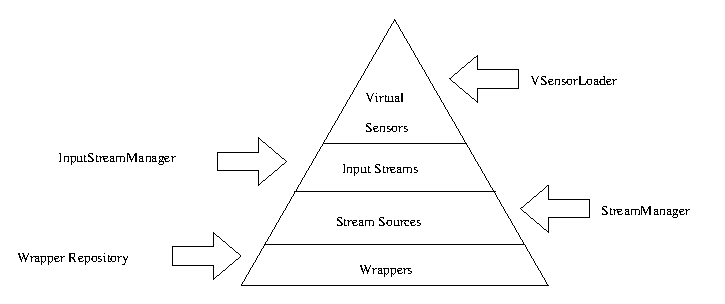
\includegraphics[width=0.5\columnwidth]{ch-gsn-figures/gsn-reuse}
  \caption{Hierarchical resource sharing in GSN}
  \label{fig:resource-layers}
\end{figure}

\textbf{Wrapper sharing.} Wrappers communicate directly with the sensors which
involves expensive I/O operations via a serial connection or wireless/wired
network communication. To minimize the costs incurred by these operations GSN
shares wrappers among virtual sensors accessing the same physical/virtual
sensors. To do so each GSN node maintains a repository of active wrappers. If a
new virtual sensor is deployed, the node first checks with the wrapper
repository whether an identical wrapper already exists, i.e., wrapper name and
initialization parameters (and their corresponding values) of the \verb|<wrapper>| element in the virtual sensor
definitions are identical. If a match is found, the new virtual sensor is
registered to the existing wrapper as a consumer. If not, a new wrapper
instance is created and registered with the wrapper repository. In the case of
remote sensor accesses this strategy is applied at both the sending and
receiving sides to maximize the sharing, i.e., multiple virtual sensors on one
GSN node share a wrapper for the same remote sensor and on the node hosting the
sensor the wrapper is shared among all nodes accessing it.

\textbf{Data sharing.} The raw input data produced by the wrappers is processed
and filtered by the source queries to generate the actual input data for the
input streams of a virtual sensor. For this purpose a source defines
what part of the raw input data is used by the associated source query
to produce the source's output data, i.e., by defining the available
storage, sampling rates, and window sizes a view on the raw data is defined on
which the source query is executed. In terms of the implementation each
wrapper is assigned a storage holding the raw data and source queries
are then defined as \emph{SQL views} on this data store.

This has a number of advantages: (1) It minimizes the storage consumption as
raw data is only stored once. Especially if the sensor data is large, e.g.,
image data, this is relevant. (2) If the sensor data comes from a
power-constrained or slow device, power is conserved and processing is sped up.
(3) Different processing strategies can be applied to the same data without
having to replicate it, for example, image enhancement algorithms and object
detection can use the same raw image data.

In the same way as a wrapper can be shared by multiple sources, a source
can also be shared among multiple streams at a higher level, and
streams in turn are shared by multiple virtual sensors. In essence each
of the layers in Figure~\ref{fig:resource-layers} can be viewed as a resource
pool where each of the individual resources in the pool can be shared among
multiple resources at the next higher level. Conversely, each higher level
resource can also use any number of lower level resources.

\subsection{Query planning and execution}
\label{sec:query-proc-optim}

In GSN each virtual sensor corresponds to a database table and each sensor
reading corresponds to a new tuple in the related table. As we use a standard
SQL database as our low-level query processing engine, the question is how to
represent the streaming logic in a form understandable for a standard database
engine (as already described, GSN separates the stream processing directives
from the query). We address this problem by using a query translator which gets
an SQL query and the stream processing directives as provided in the virtual
sensor definition as inputs and translates this into a query executable in a
standard database. The query translator relies on special support functions
which emulate stream-oriented constructs in a database. These support functions
are dependent on the database used and are provided by GSN (currently we
provide adapters for HSQLDB and MySQL). Translated queries are cached for subsequent use.

Upon deployment of a virtual sensor $VS$, all queries $Q_i$ contained in its
specification are extracted. Each query $Q_i(VS_1,\dots,VS_n)$ accesses one or
more relations $VS_1,\dots,VS_n$ which correspond to virtual sensors. Then the
query translator translates each $Q_i(VS_1,\dots,VS_n)$ into an executable
query $Q^t_i(VS_1,\dots,VS_n)$ as described above and each
$Q^t_i(VS_1,\dots,VS_n)$ is declared as a view in the database with a unique
identifier $Id_i$. This means whenever a new tuple, i.e., sensor reading, is
added to the database, the concerned views will automatically be updated by the
database. Additionally, a tuple $(VS_j, Id_i, VS)$ for each $VS_j \in
{VS_1,\dots,VS_n}$ is added to a special view registration table. This
procedure is done once when a virtual sensor is deployed.

With this setup it is now simple to execute queries over the data streams
produced by virtual sensors: As soon a new sensor reading for a virtual sensor
$VS_d$ becomes available, it is entered into the according database relation.
Then the database server queries the registration table using $VS_d$ as the key
and gets all identifiers $Id_r$ registered for new data of $VS_d$. Then simply
all views $V_r$ affected by the new data item can be retrieved using the $Id_r$
and all $V_r$ can be queried using a \texttt{SELECT * FROM} $\mathtt{V_r}$
statement and the resulting data can be returned to the virtual sensor
containing $V_r$ (third column in the registration table). Since views are
automatically updated by the database querying them is efficient. However, with
many registered views (thousands or more) scalability may suffer. Thus GSN does
not produce an individual query for each view but merges all queries into a
large select statement, and the result will then be joined with the view
registration table on the view identifier. Thus the result will hold tuples
that identify the virtual sensor to notify of the new data.  The reasons for
applying this strategy are that (1) database connections are expensive, (2)
with increasing number of clients and virtual sensor definitions, the
probability of overlaps in the result sets increases which automatically will
be exploited by the database's query processor, and (3) query execution in the
database is expensive, so one large query is much less costly than many
(possibly thousands) small ones.

Immediate notification of new sensor data is currently implemented in GSN and
is an eager strategy. As an alternative also a lazy strategy could be used
where the query execution would only take place when the GSN instance requests
it from the database, for example, periodically at regular intervals. In
practice the former can be implemented using views or triggers and the latter
can be implemented using inner selects or stored procedures.

\section{Evaluation\footnote{The evaluation results in this section correspond to GSN release 0.90.}}
\label{sec:evaluation}

GSN aims at providing a zero-programming and efficient infrastructure for
large-scale interconnected sensor networks. To justify this claim we
experimentally evaluate the throughput of the local sensor data processing and
the performance and scalability of query processing as the key influencing
factors.  As virtual sensors are addressed explicitly and GSN nodes communicate
directly in a point-to-point (peer-to-peer) style, we can reasonably
extrapolate the experimental results presented in this section to larger
network sizes.  For our experiments, we used the setup shown in
Figure~\ref{fig:ExperimentalSetup}.

The GSN network consisted of 5 standard Dell desktop PCs with Pentium 4, 3.2GHz
Intel processors with 1MB cache, 1GB memory, 100Mbit Ethernet, running Debian
3.1 Linux with an unmodified kernel 2.4.27. For the storage layer use standard
MySQL 5.18.  The PCs were attached to the following sensor networks as shown in
Figure~\ref{fig:ExperimentalSetup}.

\begin{itemize}
  
\item A sensor network consisting of 10 Mica2 motes, each mote being equipped
  with light and temperature sensors. The packet size was configured to 15
  Bytes (data portion excluding the headers).
  
\item A sensor network consisting of 8 Mica2 motes, each equipped with light,
  temperature, acceleration, and sound sensors. The packet size was
  configured to 100 Bytes (data portion excluding the headers).  The maximum
  possible packet size for TinyOS 1.x packets of the current TinyOS
  implementation is 128 bytes (including headers).
  
\item A sensor network consisting of 4 Tiny-Nodes (TinyOS compatible motes
  produced by Shockfish, \url{http://www.shockfish.com/}), each equipped with a
  light and two temperature sensors with TinyOS standard packet size of 29
  Bytes.
  
\item 15 Wireless network cameras (AXIS 206W) which can capture 640x480 JPEG
  pictures with a rate of 30 frames per second. 5 cameras use the highest
  available compression (16kB average image size), 5 use medium compression
  (32kB average image size), and 5 use no compression (75kB average image
  size). The cameras are connected to a Linksys WRT54G wireless access point
  via 802.11b and the access point is connected via 100Mbit Ethernet to a GSN
  node.
  
\item A Texas Instruments Series 6000 S6700 multi-protocol RFID reader with
  three different kind of tags, which can keep up to 8KB of data.
  128 Bytes capacity.
  
\end{itemize}

The motes in each sensor network form a sensor network and routing among the
motes is done with the surge multi-hop ad-hoc routing algorithm provided by
TinyOS.

\begin{figure}%[htb]
  \centering
  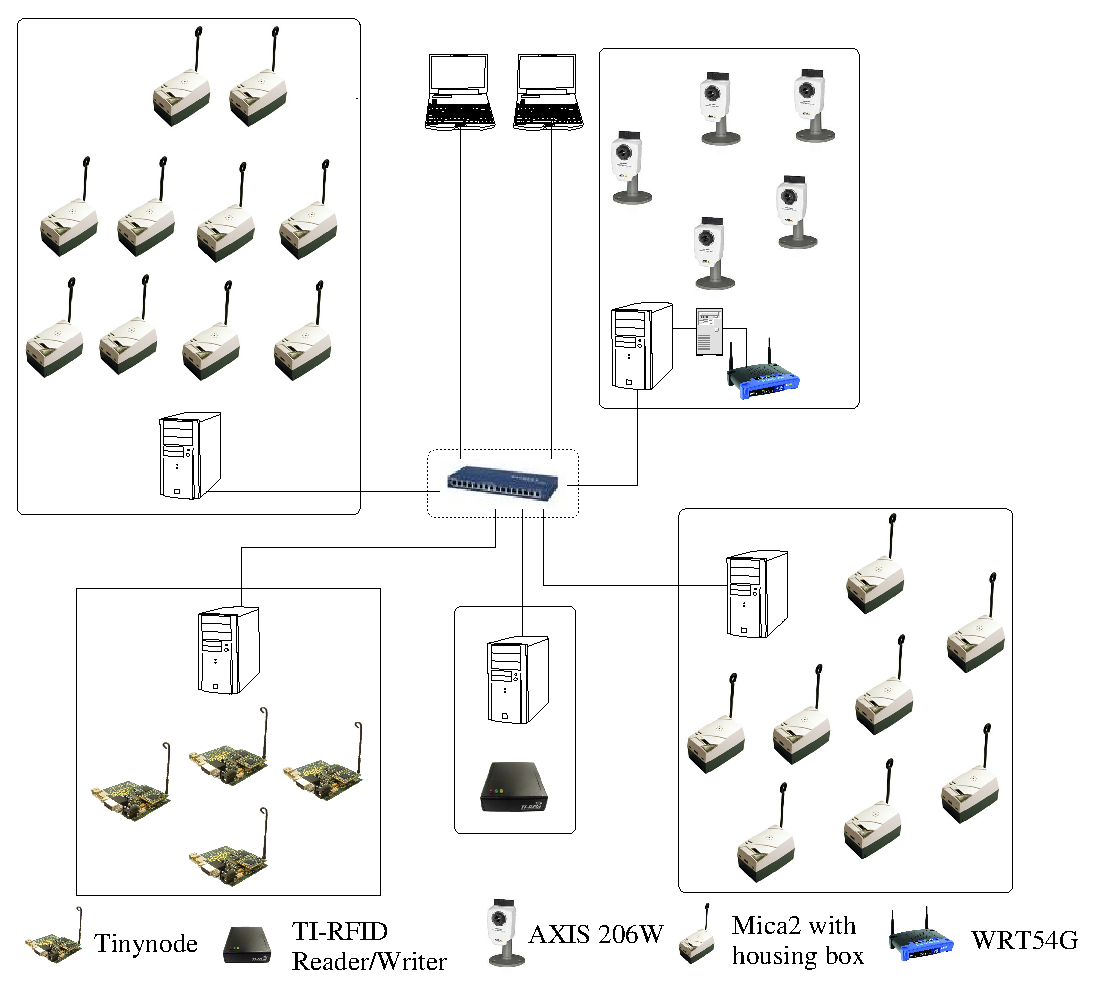
\includegraphics[width=0.8\columnwidth]{ch-gsn-figures/setup}
  \caption{Experimental setup}
  \label{fig:ExperimentalSetup}
\end{figure}


\subsection{Internal processing time}
\label{sec:exepr-eval}

In the first experiment we wanted to determine the internal processing time a
GSN node requires for processing sensor readings, i.e., the time interval when
the wrapper gets the sensor data until the data can be provided to clients by
the associated virtual sensor. This delay depends on the size of the sensor
data and the rate at which the data is produced, but is independent of the
number of clients wanting to receive the sensor data. Thus it is a lower bound
and characterizes the efficiency of the implementation. 

We configured the 22 motes and 15 cameras to produce data every 10, 25, 50,
100, 250, 500, and 1000 milliseconds. As the cameras have a maximum rate of 30
frames/second, i.e., a frame every 33 milliseconds, we added a proxy between
the GSN node and the WRT54G access point which repeated the last available
frame in order to reach a frame interval of 10 milliseconds. All GSN instances
used the Sun Java Virtual Machine (1.5.0 update 6) with memory restricted to
64MB.

The experiment was conducted as follows: All motes and cameras were set to the
same rate and produced data for 8 hours and we measured the processing delay.
This was repeated 3 times for each rate and the measurements were averaged.
Figure~\ref{fig:TimeTriggeredLoad} shows the results of the experiment for the
different data sizes produced by the motes and the cameras.

\begin{figure}%[htb]
  \centering
  \includegraphics[width=0.8\columnwidth]{ch-gsn-figures/rates}
  \caption{GSN node under time-triggered load}
  \label{fig:TimeTriggeredLoad}
\end{figure}

High data rates put some stress on the system but the absolute delays are still
quite tolerable. The delays drop sharply if the interval is increased and then
converge to a nearly constant time at a rate of approximately 4 readings/second
or less. This result shows that GSN can tolerate high rates and incurs low
overhead for realistic rates as in practical sensor deployments lower rates are
more probable due to energy constraints of the sensor devices while still being
able to deal also with high rates.


\subsection{Scalability in the number of queries and clients}
\label{sec:scal-towards-numb}

In this experiment the goal was to measure GSN's scalability in the number of
clients and queries. To do so, we used two 1.8 GHz Centrino laptops with 1GB
memory as shown in Figure~\ref{fig:ExperimentalSetup} which each ran 250
lightweight GSN instances. The lightweight GSN instance only included those
components that we needed for the experiment. Each GSN-light instance used a
random query generator to generate queries with varying table names, varying
filtering condition complexity, and varying configuration parameters such as
history size, sampling rate, etc. For the experiments we configured the query
generator to produce random queries with 3 filtering predicates in the
\texttt{where} clause on average, using random history sizes from 1 second up
to 30 minutes and uniformly distributed random sampling rates (seconds) in the
interval $[0.01,1]$.

Then we configured the motes such that they produce a measurement each second
but would deliver it with a probability $P<1$, i.e., a reading would be dropped
with probability $1-P>0$.  Additionally, each mote could produce a burst of $R$
readings at the highest possible speed depending on the hardware with
probability $B>0$, where $R$ is a uniformly random integer from the interval
$[1,100]$. I.e., a burst would occur with a probability of $P * B$ and would
produce randomly 1 up to 100 data items.  In the experiments we used $P=0.85$
and $B=0.3$. On the desktops we used MySQL as the database with the recommended
configuration for large memory systems.
Figure~\ref{fig:QueryProcessingLatency} shows the results for a stream element
size (SES) of 30 Bytes. Using SES=32KB gives the same latencies. Due
to space limitations we do not include this figure.


\begin{figure}%[htb]
  \centering
  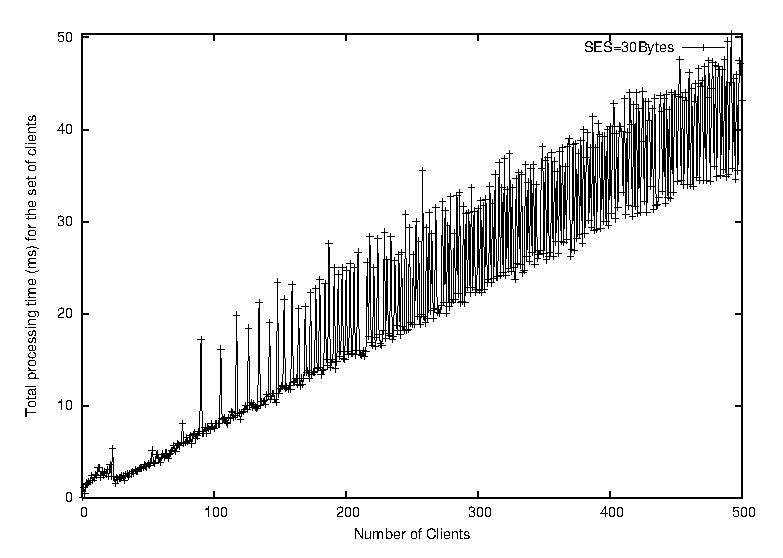
\includegraphics[width=0.8\columnwidth]{ch-gsn-figures/query-processing-time-30bytes}
%  \hspace{0.05\columnwidth}
%  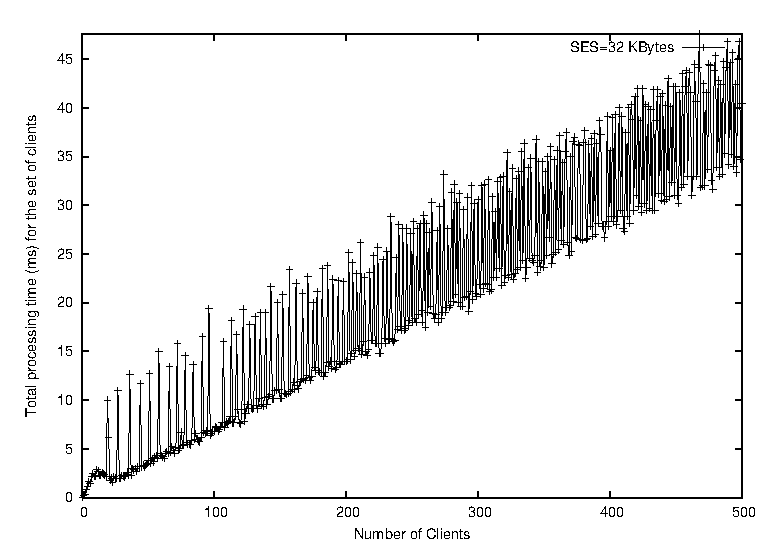
\includegraphics[width=0.45\columnwidth]{query-processing-time-32KB}
  \caption{Query processing latencies in a node}
  \label{fig:QueryProcessingLatency}
\end{figure}

The spikes in the graphs are bursts as described above. Basically this
experiment measures the performance of the database server under various loads
which heavily depends on the used database. As expected the database server's
performance is directly related to the number of the clients as with the
increasing number of clients more queries are sent to the database and also the
cost of the query compiling increases. Nevertheless, the query processing time
is reasonably low as the graphs show that the average time to process a query
if 500 clients issue queries is less than 50ms, i.e., approximately 0.5ms per
client. If required, a cluster could be used to the improve query processing
times which is supported by most of the existing databases already.

In the next experiment shown in Figure~\ref{fig:ProcessingTimePerClient} we
look at the average processing time for a client excluding the query processing
part. In this experiment we used $P=0.85$, $B=0.05$, and $R$ is as above. 

We can make three interesting observations from
Figure~\ref{fig:ProcessingTimePerClient}:

\begin{enumerate}
\item  GSN only allocates resources for virtual sensors that are being
  used. The left side of the graph shows the situation when the first
  clients arrive and use virtual sensors. The system has to instantiate
  the virtual sensor and activates the necessary resources for query
  processing, notification, connection caching, etc. Thus for the
  first clients to arrive average processing times are a bit
  higher. CPU usage is around 34\% in this interval. After a short
  time (around 30 clients) the initialization phase is over and the
  average processing time decreases as the newly arriving clients can
  already use the services in place. CPU usage then drops to around
  12\%.
  
\item Again the spikes in the graph relate to bursts. Although the processing
  time increases considerably during the bursts, the system immediately
  restores its normal behavior with low processing times when the bursts are
  over, i.e., it is very responsive and quickly adopts to varying loads.

\item As the number of clients increases, the average processing time
  for each client decreases. This is due to the implemented data
  sharing functionalities. As the number of clients increases, also
  the probability of using common resources and data items grows.
\end{enumerate}

\begin{figure}%[htb]
  \centering
  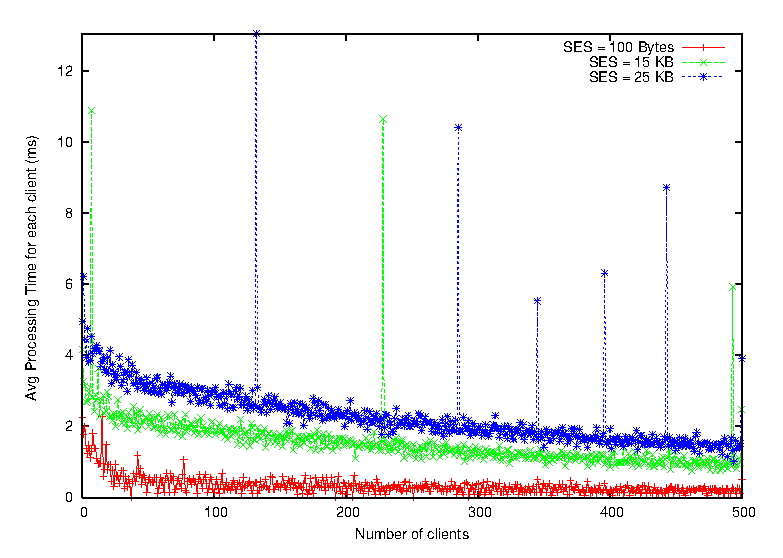
\includegraphics[width=0.8\columnwidth]{ch-gsn-figures/processing-time-per-client}
  \caption{Processing time per client}
  \label{fig:ProcessingTimePerClient}
\end{figure}

\section{Related work}
\label{sec:relatedwork}

So far only few architectures to support interconnected sensor networks exist.
Sgroi et al.~\cite{Sgroi05} suggest basic abstractions, a standard set of
services, and an API to free application developers from the details of the
underlying sensor networks.  However, the focus is on systematic definition and
classification of abstractions and services, while GSN takes a more general
view and provides not only APIs but a complete query processing and management
infrastructure with a declarative language interface.

Hourglass~\cite{Shneidman04} provides an Internet-based infrastructure for
connecting sensor networks to applications and offers topic-based discovery and
data-processing services. Similar to GSN it tries to hide internals of sensors
from the user but focuses on maintaining quality of service of data streams in
the presence of disconnections while GSN is more targeted at flexible
configurations, general abstractions, and distributed query support.

HiFi~\cite{Franklin05} provides efficient, hierarchical data stream query
processing to acquire, filter, and aggregate data from multiple devices in a
static environment while GSN takes a peer-to-peer perspective assuming a
dynamic environment and allowing any node to be a data source, data sink, or
data aggregator.

IrisNet~\cite{Gibbons03} proposes a two-tier architecture consisting of sensing
agents (SA) which collect and pre-process sensor data and organizing agents
(OA) which store sensor data in a hierarchical, distributed XML database. This
database is modeled after the design of the Internet DNS and supports XPath
queries. In contrast to that, GSN follows a symmetric peer-to-peer approach as
already mentioned and supports relational queries using SQL.

Rooney et al.~\cite{Rooney06} propose so-called EdgeServers to integrate sensor
networks into enterprise networks. EdgeServers filter and aggregate raw sensor
data (using application specific code) to reduce the amount of data forwarded
to application servers. The system uses publish/subscribe style communication
and also includes specialized protocols for the integration of sensor
networks. While GSN provides a general-purpose infrastructure for sensor
network deployment and distributed query processing, the EdgeServer system
targets enterprise networks with application-based customization to reduce
sensor data traffic in closed environments.

Besides these architectures, a large number of systems for query processing in
sensor networks exist. Aurora~\cite{Cherniack03} (Brandeis University, Braun
University, MIT), STREAM~\cite{Arasu06} (Stanford),
TelegraphCQ~\cite{Chandrasekaran03} (UC Berkeley), and Cougar~\cite{Yao03}
(Cornell) have already been discussed and related to GSN in
Section~\ref{sec:data-stre-proc}.

%The Aurora project~\cite{Cherniack03} is a general-purpose centralized stream
%processing engine. Streams are modeled as sequences of time-stamped tuples, and
%users can compose stream relationships and construct queries in a graphical
%representation which is then used as input for the query planner.

In the Medusa distributed stream-processing system~\cite{Zdonik03}, Aurora is
being used as the processing engine on each of the participating nodes. Medusa
takes Aurora queries and distributes them across multiple nodes and
particularly focuses on load management using economic principles and high
availability issues. The Borealis stream processing engine~\cite{Abadi05} is
based on the work in Medusa and Aurora and supports dynamic query modification,
dynamic revision of query results, and flexible optimization. These systems
focus on (distributed) query processing only, which is only one specific
component of GSN, and focus on sensor heavy and server heavy application
domains.

Additionally, several systems providing publish/subscribe-style query
processing comparable to GSN exist, for example, \cite{Gray05}.

\section{Conclusions}
\label{sec:conclusions}

The full potential of sensor technology will be unleashed through large-scale
(up to global scale) data-oriented integration of sensor networks. To realize
this vision of a ``Sensor Internet'' we suggest our Global Sensor Networks
(GSN) middleware which enables fast and flexible deployment and interconnection
of sensor networks. Through its virtual sensor abstraction which can abstract
from arbitrary stream data sources and its powerful declarative specification
and query tools, GSN provides simple and uniform access to the host of
heterogeneous technologies. GSN offers zero-programming deployment and
data-oriented integration of sensor networks and supports dynamic configuration
and adaptation at runtime. Zero-programming deployment in conjunction with
GSN's plug-and-play detection and deployment feature provides a basic
functionality to enable sensor mobility. GSN is implemented in Java and C/C++
and is available from SourceForge at \url{http://gsn.sourcefourge.net/}.
The experimental evaluation of GSN demonstrates that the implementation is
highly efficient, offers very good performance and throughput even under high
loads and scales gracefully in the number of nodes, queries, and query
complexity.



	%
	%\chapter{{\LaTeX} Examples}


\begin{table*}[!htp]
	\centering
	{\normalfont\footnotesize
	\begin{tabulary}{\textwidth}{|C|C|C|C|J|}%
	\hline
		\multicolumn{5}{|c|}{\textbf{Parameters for example Wrapper (that support safe storage)}} \\
	\hline
	\hline
		\textbf{Parameter Name} &
		\textbf{Type} &
		\textbf{Mandatory} &
		\textbf{Default} &
		\textbf{Description} \\
	\hline
	\hline
		param1 &
		String &	
		Yes &
		None &
		param1 description \\
	\hline
		\multicolumn{5}{|l|}{This Wrapper supports Safe Storage. Parameters listed on \tableref{table:safe_storage_parameters} must be added.} \\
	\hline
	\end{tabulary}
	}
	\caption{Parameters for example Wrapper (that support safe storage)}
	\label{table:parameters_example_wrapper}
\end{table*}

\begin{table*}[!htp]
	\centering
	{\normalfont\footnotesize
	\begin{tabulary}{\textwidth}{|C|C|C|C|J|}%
	\hline
		\multicolumn{5}{|c|}{\textbf{Parameters for example Wrapper (that doensn't support safe storage)}} \\
	\hline
	\hline
		\textbf{Parameter Name} &
		\textbf{Type} &
		\textbf{Mandatory} &
		\textbf{Default} &
		\textbf{Description} \\
	\hline
	\hline
		param1 &
		String &	
		Yes &
		None &
		param1 description \\
	\hline
	param2 &
		String &	
		Yes &
		None &
		param2 description \\
	\hline
	\end{tabulary}
	}
	\caption{Parameters for example Wrapper (that doensn't support safe storage)}
	\label{table:parameters_example_no_wrapper}
\end{table*}


\begin{rubycode}[caption={Ruby Code Example}, label=listing:ruby:example]
# A method
def mymethod 
	@foo.each { |bar| bar.to_s }
	@@foobar = "a string"
end
\end{rubycode}

\begin{javacode}
/**
 * Java Class
 */
public class Test {
	private int test;
	public Test () {}
	public Test (int level) {
		// A comment
		String b = "my test string";
		this.test = test;
	}
}
\end{javacode}

\begin{xmlcode}[caption={XML Code Example}, label=listing:xml:example]
<!-- one comment -->
<tag attribute="val1">
	<tag2 p="5" />
</tag>
\end{xmlcode}

\begin{htmlcode}
<!-- one comment -->
<html>
	<head>
		<title>Test Page</title>
	</head>
	<body>
		<p style="display: none;">Test</p>
	</body>
</html>
\end{htmlcode}

citation \cite{dummyarticle}

\url{http://www.google.ch}
\href{http://www.google.ch}{www.google.ch}


	
%	\bibliography{GSN}
\end{document}
